\section{Results} \label{sec:results}

\subsection{Data analysis algorithm}

Data analysis was performed in the following steps:
\begin{enumerate}
\item calculate log returns of the input data to make time series stationary,
\item decompose log returns in Daubechies (\emph{db4} in PyWavelet implementation) wavelet basis,
\item reconstruct data in the original domain for each time scale,
\item test for linear Granger causality using an autoregressive model test between each wavelet scale pair, for up to 5 steps,
\item test for nonlinear Granger causality using the Diks-Panchenko test between each wavelet scale pair, for up to 5 steps.
\end{enumerate}

Then, 1000 surrogate data sets were generated with phase randomisation method as described in \fref{sec:surrogate-method} and the same analysis procedure was perfomed for each realization.
The number of statistically significant results among surrogates divided by number of realizations was used to asses results fidelity.

Statistical significance was assumed for $p$-values less than $0.05$ for both linear and nonlinear tests.

Given 552 monthly observations (45 years) in the analyzed data sets, the wavelet scales correspond to the time scales as presented in \fref{tab:scales} 

\begin{table}[h]
\begin{center}
\begin{tabular}{c|c}
\hline\hline
Wavelet scale & Time scale \\
\hline
D1 & 2-4 months \\
D2 & 4-8 months \\
D3 & 8-16 months \\
D4 & 16-32 months \\
D5 & 32-64 months \\
D6 & 64-128 months \\
A6 & $>$128 months \\
\hline\hline
\end{tabular}
\end{center}
\caption{Wavelet time scales}
\label{tab:scales}
\end{table}

\newpage
\subsection{Wavelet decomposed data}
Logarithmic returns of the time series are presented in \ref{fig:usd-logret} and \ref{fig:oil-logret}.
Wavelet decomposition of the original data is presented here in figures: \ref{fig:usd-wr-a6}-\ref{fig:oil-wr-d6}.
To depict how different wavelet scales relate to the input data, the logarithmic returns are displayed in light grey in the background of each plot.
An example of generated surrogate data and its wavelet decomposition is presented in \fref{appendix:surrogate-example}.

\begin{figure}[h]
\begin{center}
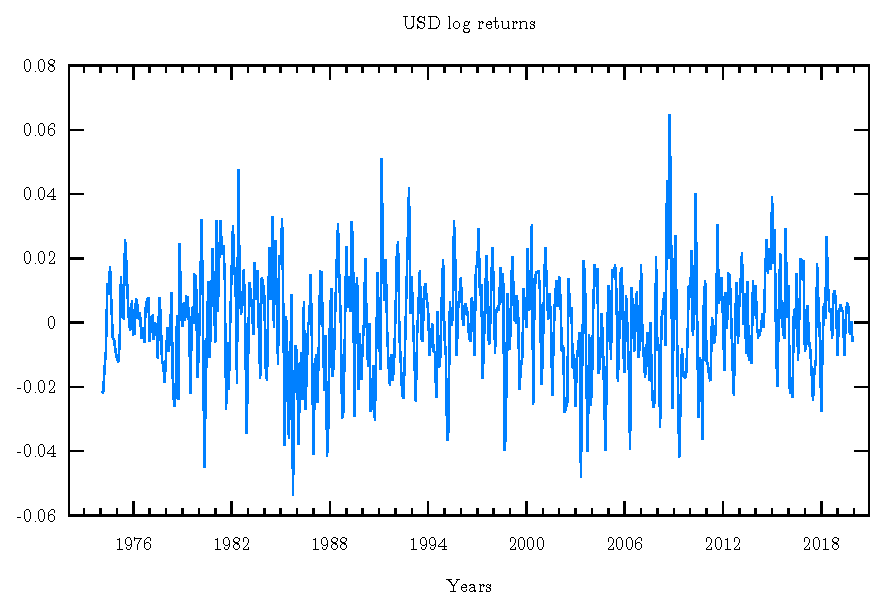
\includegraphics[width=0.8\textwidth]{./code/plot/dollar_logret.eps}
\caption{Plot of log returns of U.S. Dollar Index.}
\label{fig:usd-logret}
\end{center}
\end{figure}

\begin{figure}
\begin{center}
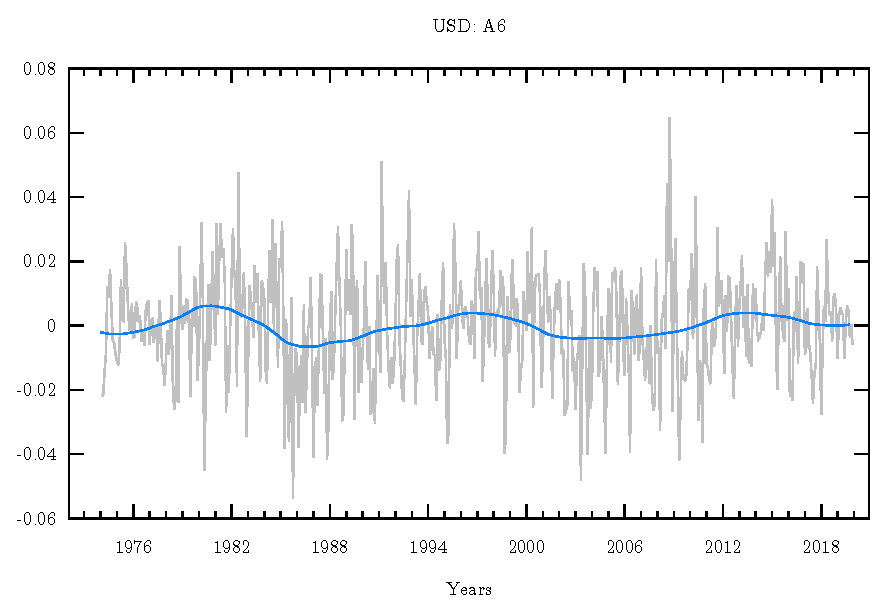
\includegraphics[width=0.8\textwidth]{./code/plot/usd_wr_A6.eps}
\caption{Plot of A6 component of wavelet decomposition of U.S. Dollar Index log returns. 
	Plot of the original data in grey. A6 scale corresponds to $>$128 months.}
\label{fig:usd-wr-a6}
\end{center}
\end{figure}

\begin{figure}
\begin{center}
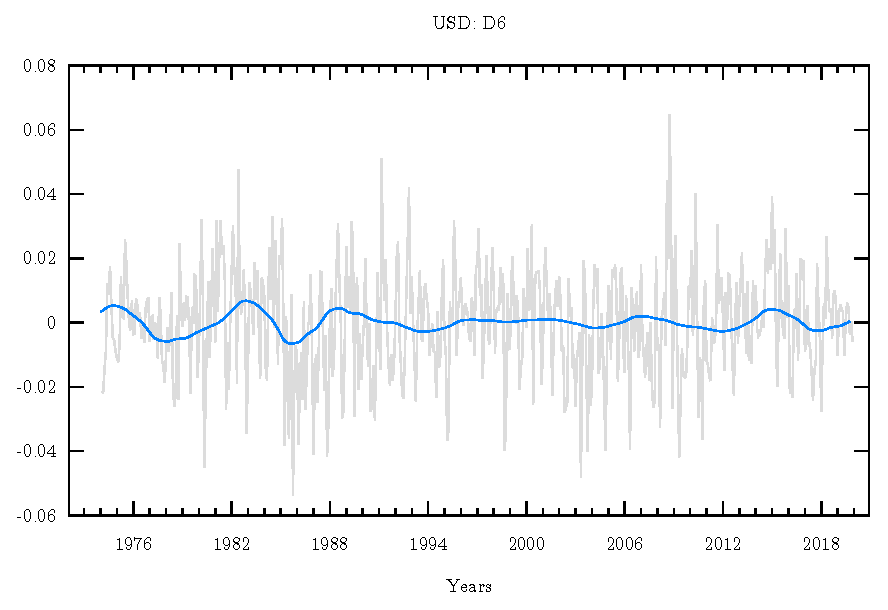
\includegraphics[width=0.8\textwidth]{./code/plot/usd_wr_D6.eps}
\caption{Plot of D6 component of wavelet decomposition of U.S. Dollar Index log returns. 
	Plot of the original data in grey. D6 scale corresponds to 64-128 months.}
\label{fig:usd-wr-d6}
\end{center}
\end{figure}

\begin{figure}
\begin{center}
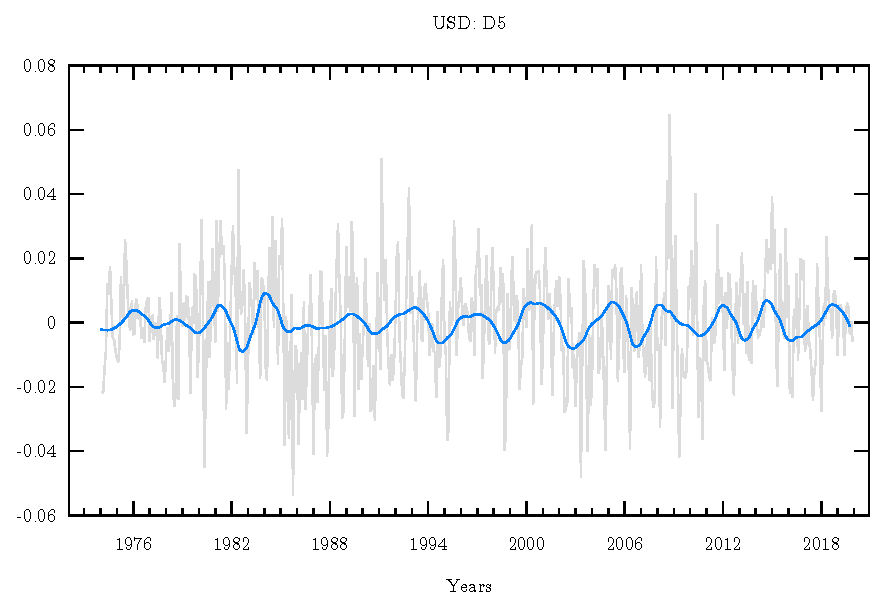
\includegraphics[width=0.8\textwidth]{./code/plot/usd_wr_D5.eps}
\caption{Plot of D5 component of wavelet decomposition of U.S. Dollar Index log returns. 
	Plot of the original data in grey. D5 scale corresponds to 32-64 months.}
\label{fig:usd-wr-d5}
\end{center}
\end{figure}

\begin{figure}
\begin{center}
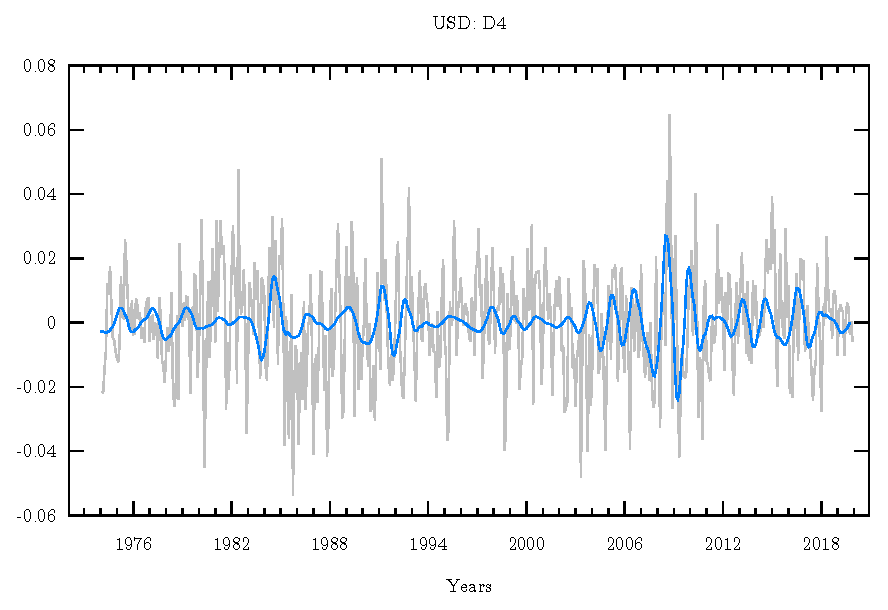
\includegraphics[width=0.8\textwidth]{./code/plot/usd_wr_D4.eps}
\caption{Plot of D4 component of wavelet decomposition of U.S. Dollar Index log returns. 
	Plot of the original data in grey. D4 scale corresponds to 16-32 months.}
\label{fig:usd-wr-d4}
\end{center}
\end{figure}

\begin{figure}
\begin{center}
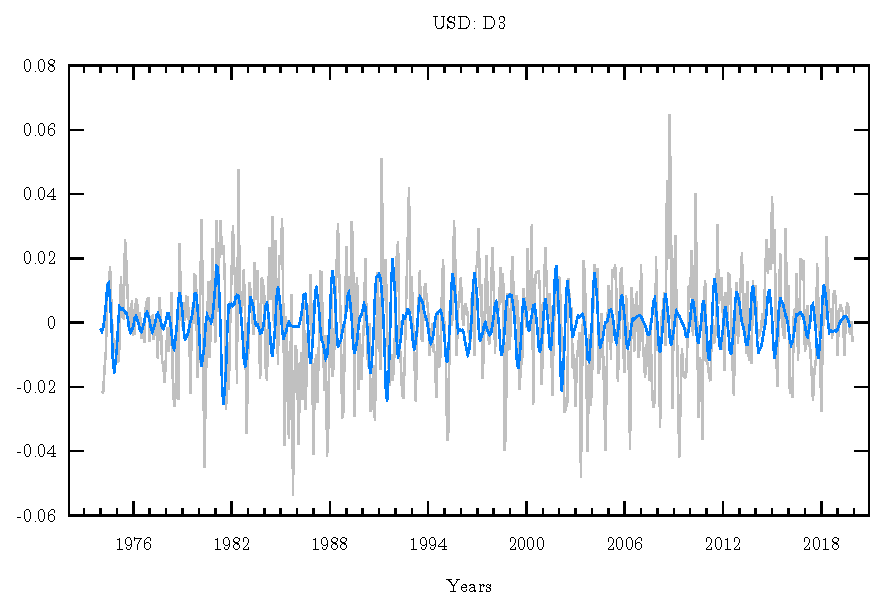
\includegraphics[width=0.8\textwidth]{./code/plot/usd_wr_D3.eps}
\caption{Plot of D3 component of wavelet decomposition of U.S. Dollar Index log returns. 
	Plot of the original data in grey. D3 scale corresponds to 8-16 months.}
\label{fig:usd-wr-d3}
\end{center}
\end{figure}

\begin{figure}
\begin{center}
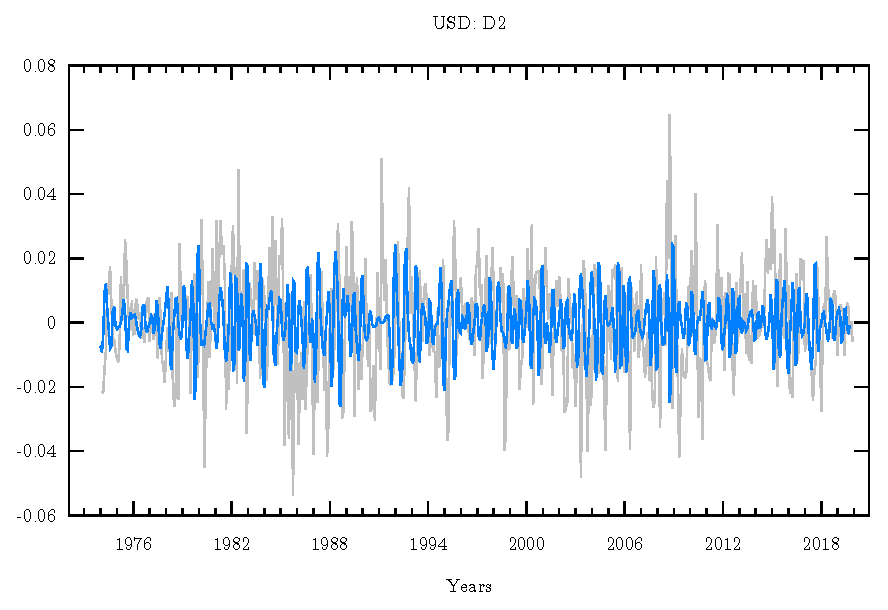
\includegraphics[width=0.8\textwidth]{./code/plot/usd_wr_D2.eps}
\caption{Plot of D2 component of wavelet decomposition of U.S. Dollar Index log returns. 
	Plot of the original data in grey. D2 scale corresponds to 4-8 months.}
\label{fig:usd-wr-d2}
\end{center}
\end{figure}

\begin{figure}
\begin{center}
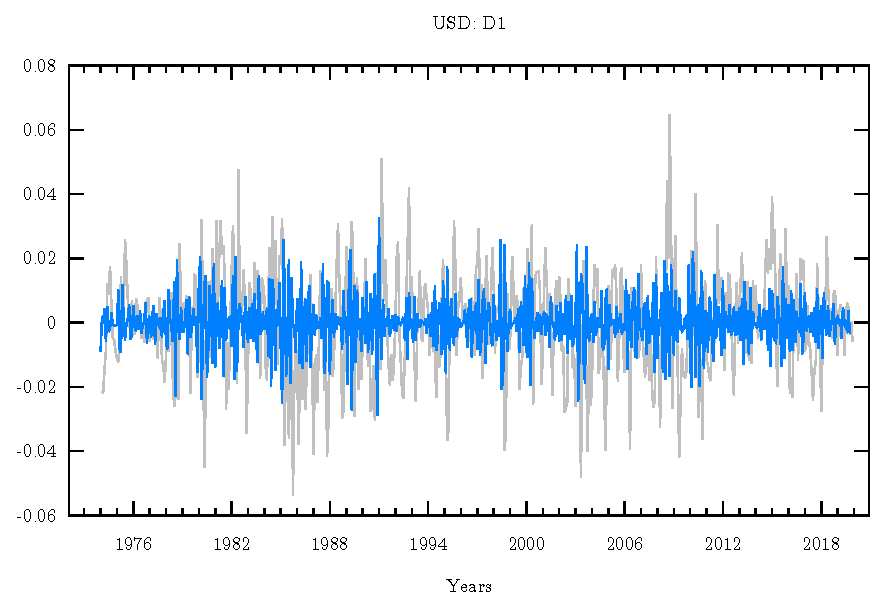
\includegraphics[width=0.8\textwidth]{./code/plot/usd_wr_D1.eps}
\caption{Plot of D1 component of wavelet decomposition of U.S. Dollar Index log returns. 
	Plot of the original data in grey. D1 scale corresponds to 2-4 months.}
\label{fig:usd-wr-d1}
\end{center}
\end{figure}

\begin{figure}
\begin{center}
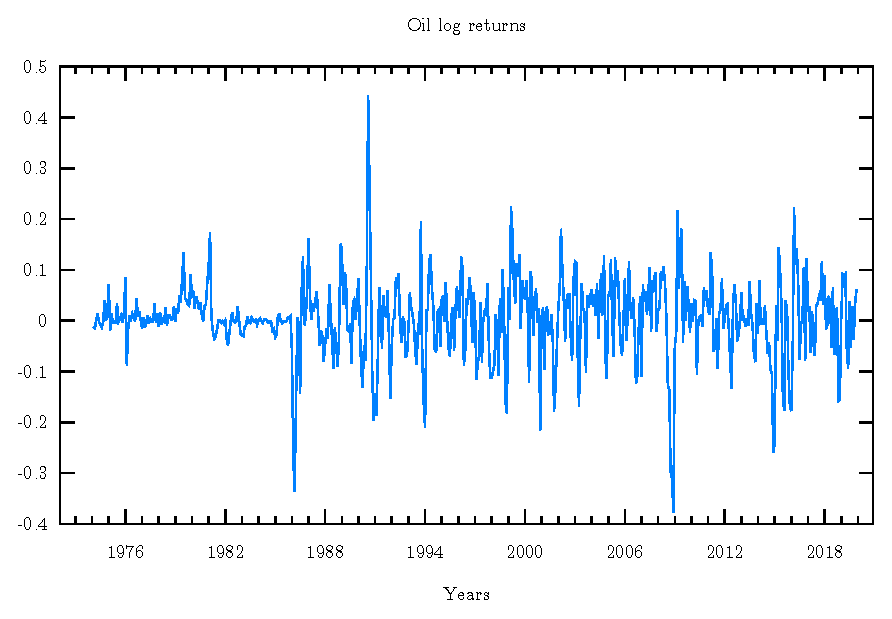
\includegraphics[width=0.8\textwidth]{./code/plot/oil_logret.eps}
\caption{Plot of log returns of oil price.}
\label{fig:oil-logret}
\end{center}
\end{figure}

\begin{figure}
\begin{center}
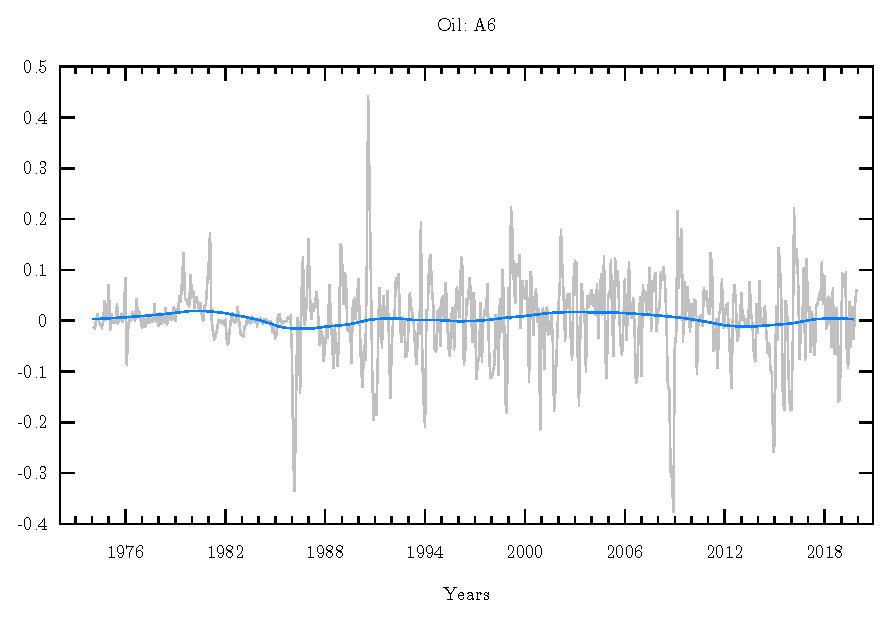
\includegraphics[width=0.8\textwidth]{./code/plot/oil_wr_A6.eps}
\caption{Plot of A6 component of wavelet decomposition oil price  log returns. 
	Plot of the original data in grey. A6 scale corresponds to $>$128 months.}
\label{fig:oil-wr-a6}
\end{center}
\end{figure}

\begin{figure}
\begin{center}
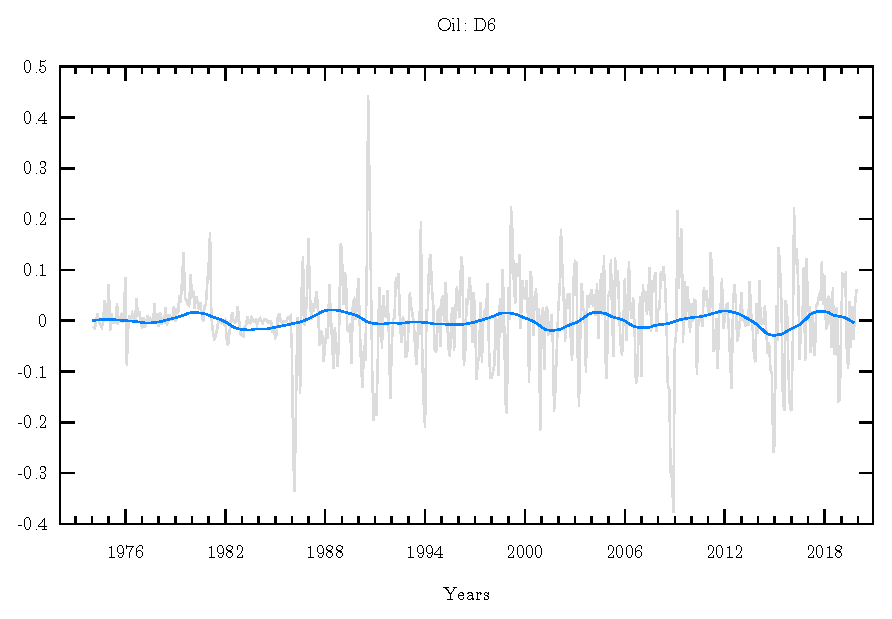
\includegraphics[width=0.8\textwidth]{./code/plot/oil_wr_D6.eps}
\caption{Plot of D6 component of wavelet decomposition of oil price log returns. 
	Plot of the original data in grey. D6 scale corresponds to 64-128 months.}
\label{fig:oil-wr-d6}
\end{center}
\end{figure}

\begin{figure}
\begin{center}
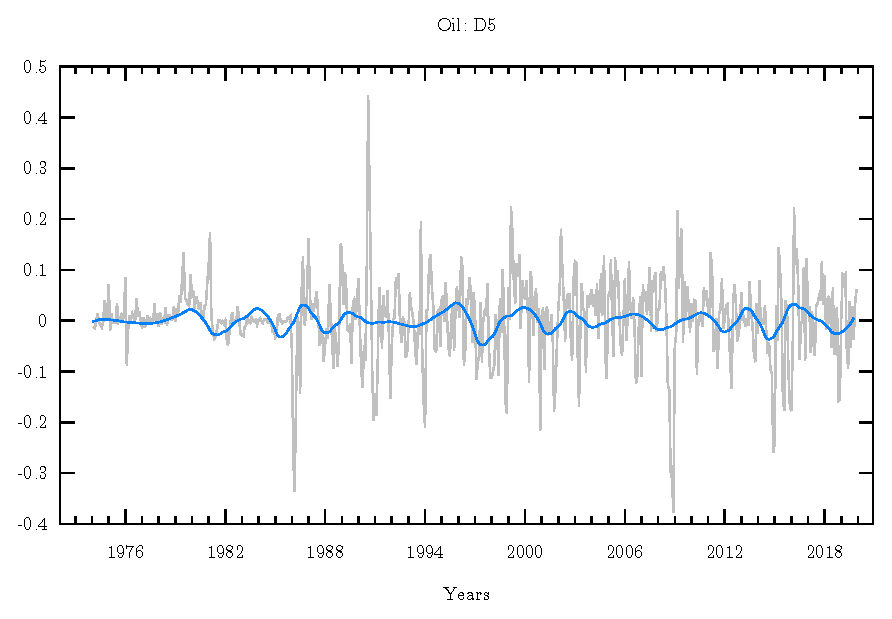
\includegraphics[width=0.8\textwidth]{./code/plot/oil_wr_D5.eps}
\caption{Plot of D5 component of wavelet decomposition of oil price log returns. 
	Plot of the original data in grey. D5 scale corresponds to 32-64 months.}
\label{fig:oil-wr-d5}
\end{center}
\end{figure}

\begin{figure}
\begin{center}
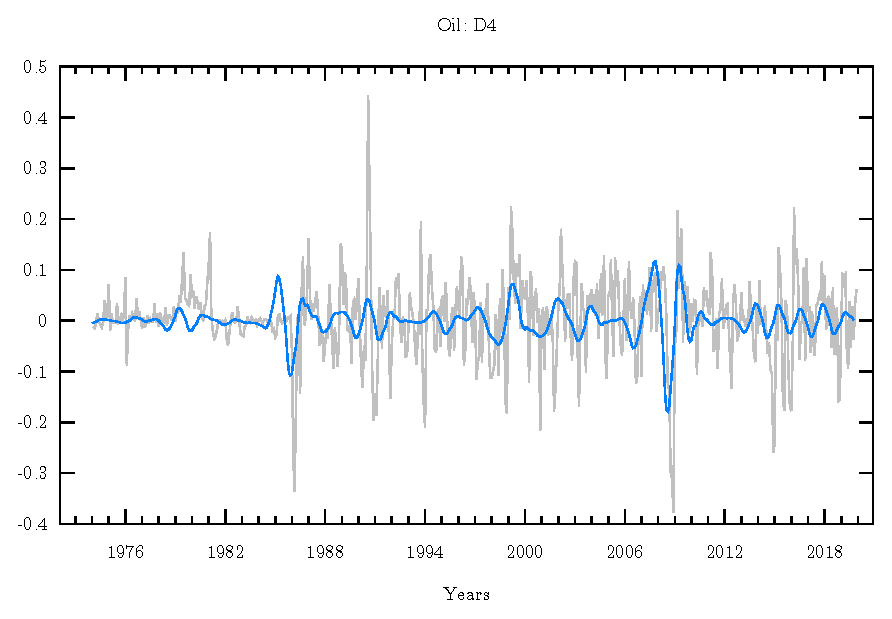
\includegraphics[width=0.8\textwidth]{./code/plot/oil_wr_D4.eps}
\caption{Plot of D4 component of wavelet decomposition of oil price log returns. 
	Plot of the original data in grey. D4 scale corresponds to 16-32 months.}
\label{fig:oil_wr_d4}
\end{center}
\end{figure}

\begin{figure}
\begin{center}
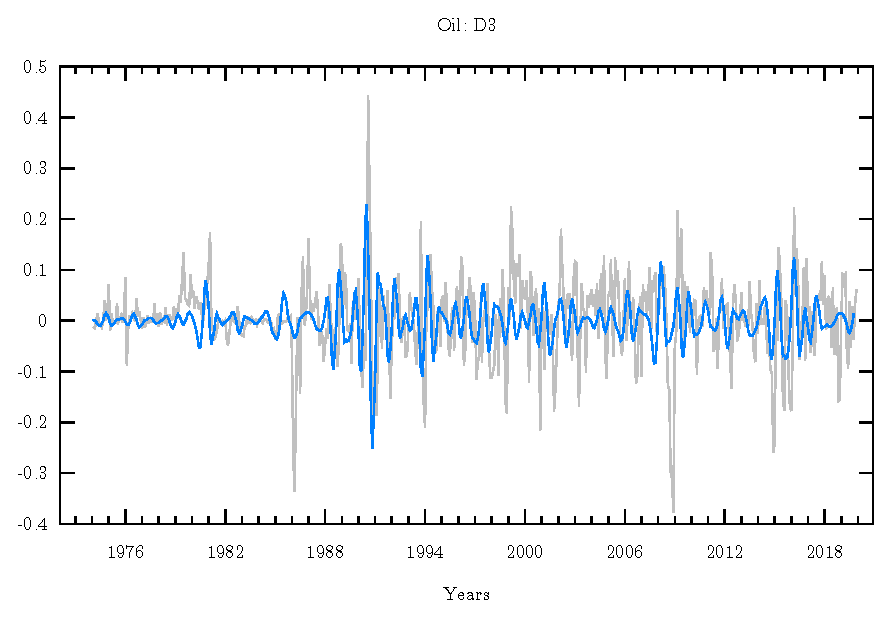
\includegraphics[width=0.8\textwidth]{./code/plot/oil_wr_D3.eps}
\caption{Plot of D3 component of wavelet decomposition of oil price log returns. 
	Plot of the original data in grey. D3 scale corresponds to 8-16 months.}
\label{fig:oil-wr-d3}
\end{center}
\end{figure}

\begin{figure}
\begin{center}
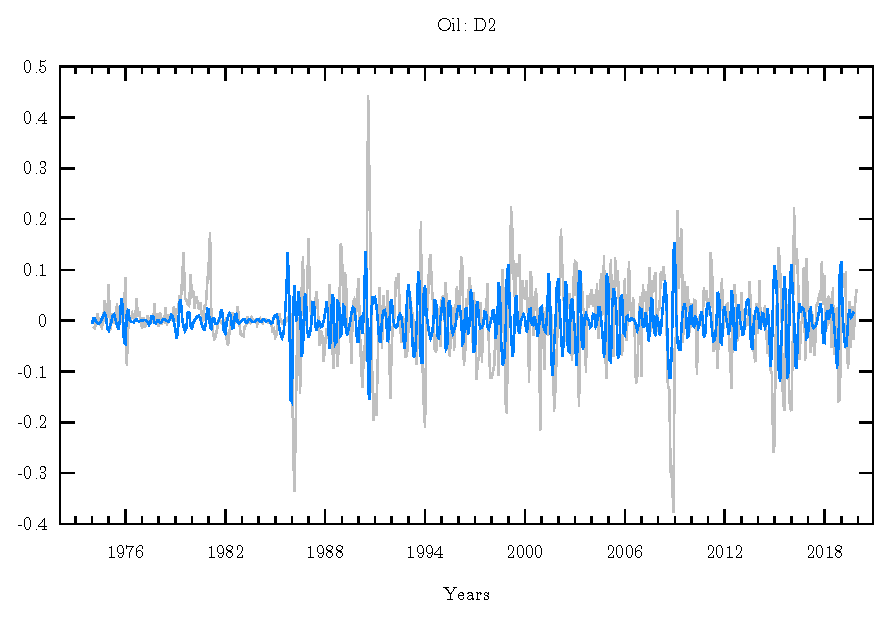
\includegraphics[width=0.8\textwidth]{./code/plot/oil_wr_D2.eps}
\caption{Plot of D2 component of wavelet decomposition of oil price log returns. 
	Plot of the original data in grey. D2 scale corresponds to 4-8 months.}
\label{fig:oil-wr-d2}
\end{center}
\end{figure}

\begin{figure}
\begin{center}
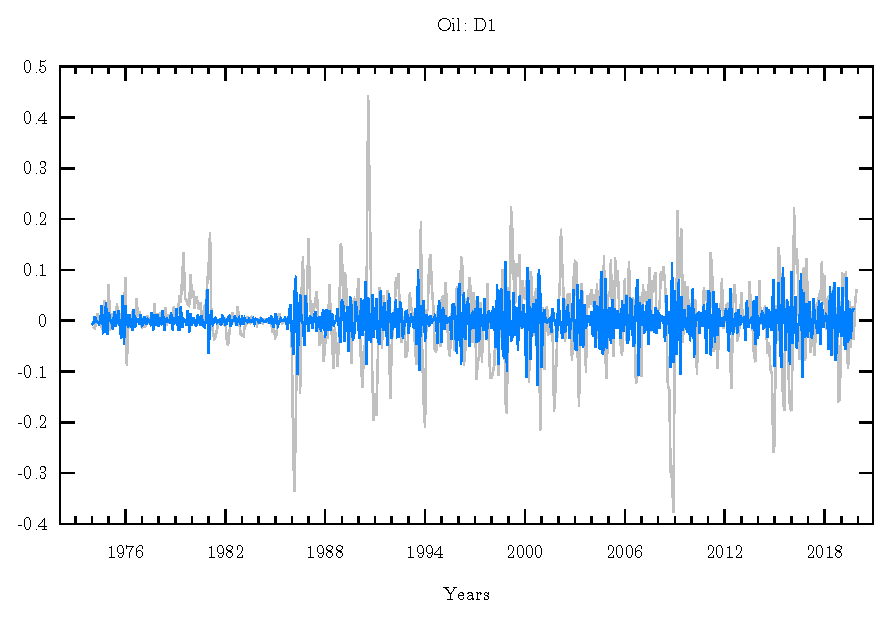
\includegraphics[width=0.8\textwidth]{./code/plot/oil_wr_D1.eps}
\caption{Plot of D1 component of wavelet decomposition of oil price log returns. 
	Plot of the original data in grey. D1 scale corresponds to 2-4 months.}
\label{fig:oil-wr-d1}
\end{center}
\end{figure}

\newpage
\subsection{Causality tests results}

\subsubsection{Linear causality test results}

%
% USD A6 -> OIL
%
\begin{table}[H]
\begin{center}
\begin{tabular}{l|r r r r r r r}
\hline\hline
\multicolumn{8}{c}{USD $\Rightarrow$ Oil}\\
\hline
\multicolumn{8}{c}{Causality from A6}\\
\hline\hline
m & A6 & D6 & D5 & D4 & D3 & D2 & D1 \\
\hline
1 & 0.6200 & \cellcolor{mygreen}0.0001 & 0.6100 & 0.9875 & 0.9993 & 0.9998 & 0.9935 \\
2 & 0.3321 & \cellcolor{mygreen}0.0077 & 0.6439 & 0.9943 & 0.9993 & 0.9998 & 0.9999 \\
3 & 0.7979 & 0.2591 & 0.9150 & 0.9994 & 0.9968 & 0.9996 & 0.8537 \\
4 & 0.8756 & 0.1705 & 0.7704 & 1.0000 & 0.9760 & 0.9999 & 0.5546 \\
5 & 0.8545 & 0.2808 & 0.7016 & 1.0000 & 0.9923 & 0.9999 & 0.8883 \\
6 & 0.8272 & 0.1676 & 0.7324 & 1.0000 & 0.9647 & 0.9966 & 0.9674 \\
\hline\hline
\end{tabular}
\caption{p-values for linear Granger causality test under $H_0$:\\
U.S. Dollar Index A6 band does not cause oil price. Statistical significance assumed for $p<0.05$.} 
\end{center}
\end{table}

%
% USD D6 -> OIL
%
\begin{table}[H]
\begin{center}
\begin{tabular}{l|r r r r r r r}
\hline\hline
\multicolumn{8}{c}{USD $\Rightarrow$ Oil}\\
\hline
\multicolumn{8}{c}{Causality from D6}\\
\hline\hline
m & A6 & D6 & D5 & D4 & D3 & D2 & D1 \\
\hline
1 & 0.2686 & \cellcolor{mygreen}0.0000 & 0.8785 & 0.5212 & 0.9635 & 0.9912 & 0.9906 \\
2 & \cellcolor{mygreen}0.0164 & 0.3609 & 0.8507 & 0.4577 & 0.9619 & 0.9989 & 0.9994 \\
3 & 0.2598 & 0.7244 & 0.9835 & 0.7008 & 0.9602 & 1.0000 & 0.6645 \\
4 & 0.3306 & 0.6557 & 0.9927 & 0.5924 & 0.7660 & 0.9979 & 0.4818 \\
5 & 0.5460 & 0.6330 & 0.9982 & 0.1360 & 0.8186 & 0.9996 & 0.8271 \\
6 & 0.3874 & 0.7689 & 0.9913 & 0.0524 & 0.8126 & 0.9722 & 0.9743 \\
\hline\hline
\end{tabular}
\caption{p-values for linear Granger causality test under $H_0$:\\
U.S. Dollar Index D6 band does not cause oil price. Statistical significance assumed for $p<0.05$.}
\end{center}
\end{table}

%
% USD D5 -> OIL
%
\begin{table}[H]
\begin{center}
\begin{tabular}{l|r r r r r r r}
\hline\hline
\multicolumn{8}{c}{USD $\Rightarrow$ Oil}\\
\hline
\multicolumn{8}{c}{Causality from D5}\\
\hline\hline
m & A6 & D6 & D5 & D4 & D3 & D2 & D1 \\
\hline
1 & \cellcolor{mygreen}0.0454 & \cellcolor{mygreen}0.0000 & \cellcolor{mygreen}0.0000 & 0.2192 & 0.8601 & 0.9319 & 0.9999 \\
2 & 0.7743 & 0.3405 & 0.4076 & 0.3828 & 0.8463 & 0.9366 & 0.9906 \\
3 & 0.9822 & 0.4960 & 0.6347 & 0.7134 & 0.9232 & 0.3698 & 0.7828 \\
4 & 0.9105 & 0.6575 & 0.7249 & 0.5834 & 0.8687 & 0.7226 & 0.4026 \\
5 & 0.9268 & 0.5320 & 0.3842 & 0.7342 & 0.8616 & 0.6901 & 0.4900 \\
6 & 0.9592 & 0.5967 & 0.2039 & 0.6918 & 0.9815 & 0.9510 & 0.5241 \\
\hline\hline
\end{tabular}
\caption{p-values for linear Granger causality test under $H_0$:\\
U.S. Dollar Index D5 band does not cause oil price. Statistical significance assumed for $p<0.05$.}
\end{center}
\end{table}

%
% USD D4 -> OIL
%
\begin{table}[H]
\begin{center}
\begin{tabular}{l|r r r r r r r}
\hline\hline
\multicolumn{8}{c}{USD $\Rightarrow$ Oil}\\
\hline
\multicolumn{8}{c}{Causality from D4}\\
\hline\hline
m & A6 & D6 & D5 & D4 & D3 & D2 & D1 \\
\hline
1 & 0.2897 & 0.9118 & 0.4934 & 0.9984 & 0.2238 & 0.8936 & 0.9500 \\
2 & 0.4679 & \cellcolor{mygreen}0.0000 & 0.9642 & 0.0964 & 0.0942 & 0.9349 & 0.9433 \\
3 & 0.8458 & \cellcolor{mygreen}0.0000 & 0.9950 & 0.3228 & 0.1420 & 0.8259 & 0.5060 \\
4 & 0.8966 & \cellcolor{mygreen}0.0000 & 0.9983 & 0.1069 & 0.1400 & 0.9318 & 0.1855 \\
5 & 0.3120 & \cellcolor{mygreen}0.0000 & 0.9997 & 0.4028 & 0.1501 & 0.9578 & 0.1915 \\
6 & 0.1033 & \cellcolor{mygreen}0.0000 & 0.9999 & 0.1459 & 0.0981 & 0.9892 & 0.4155 \\
\hline\hline
\end{tabular}
\caption{p-values for linear Granger causality test under $H_0$:\\
U.S. Dollar Index D4 band does not cause oil price. Statistical significance assumed for $p<0.05$.}
\end{center}
\end{table}

%
% USD D3 -> OIL
%
\begin{table}[H]
\begin{center}
\begin{tabular}{l|r r r r r r r}
\hline\hline
\multicolumn{8}{c}{USD $\Rightarrow$ Oil}\\
\hline
\multicolumn{8}{c}{Causality from D3}\\
\hline\hline
m & A6 & D6 & D5 & D4 & D3 & D2 & D1 \\
\hline
1 & 0.5554 & 0.7389 & 0.2930 & 0.2254 & 0.3766 & \cellcolor{mygreen}0.0293 & 0.9490 \\
2 & 0.3045 & 0.5258 & 0.7617 & 0.7649 & 0.3534 & \cellcolor{mygreen}0.0061 & 0.8265 \\
3 & 0.2833 & 0.7572 & 0.9259 & 0.9097 & 0.4805 & \cellcolor{mygreen}0.0038 & 0.2173 \\
4 & \cellcolor{mygreen}0.0031 & 0.7637 & 0.0946 & 0.8202 & 0.5700 & \cellcolor{mygreen}0.0134 & \cellcolor{mygreen}0.0468 \\
5 & \cellcolor{mygreen}0.0016 & 0.8090 & 0.1489 & 0.9177 & 0.3863 & \cellcolor{mygreen}0.0166 & 0.1471 \\
6 & \cellcolor{mygreen}0.0028 & 0.9388 & 0.1538 & 0.9465 & 0.5367 & \cellcolor{mygreen}0.0014 & \cellcolor{mygreen}0.0417 \\
\hline\hline
\end{tabular}
\caption{p-values for linear Granger causality test under $H_0$:\\
U.S. Dollar Index D3 band does not cause oil price. Statistical significance assumed for $p<0.05$.}
\end{center}
\end{table}

%
% USD D2 -> OIL
%
\begin{table}[H]
\begin{center}
\begin{tabular}{l|r r r r r r r}
\hline\hline
\multicolumn{8}{c}{USD $\Rightarrow$ Oil}\\
\hline
\multicolumn{8}{c}{Causality from D2}\\
\hline\hline
m & A6 & D6 & D5 & D4 & D3 & D2 & D1 \\
\hline
1 & 0.9326 & 0.7834 & 0.5304 & 0.6002 & 0.9506 & 0.0569 & \cellcolor{mygreen}0.0087 \\
2 & 0.4000 & 0.4564 & 0.2379 & \cellcolor{mygreen}0.0153 & 0.5042 & 0.4186 & \cellcolor{mygreen}0.0212 \\
3 & 0.3273 & 0.3233 & \cellcolor{mygreen}0.0136 & \cellcolor{mygreen}0.0274 & 0.5943 & 0.2531 & 0.0827 \\
4 & 0.5227 & 0.5441 & 0.0821 & 0.2043 & 0.7386 & 0.3128 & 0.5504 \\
5 & 0.6493 & 0.2822 & \cellcolor{mygreen}0.0163 & 0.2737 & 0.7311 & 0.3002 & \cellcolor{mygreen}0.0033 \\
6 & 0.4422 & 0.0911 & 0.1994 & 0.1045 & 0.9044 & 0.5168 & \cellcolor{mygreen}0.0164 \\
\hline\hline
\end{tabular}
\caption{p-values for linear Granger causality test under $H_0$:\\
U.S. Dollar Index D2 band does not cause oil price. Statistical significance assumed for $p<0.05$.}
\end{center}
\end{table}

%
% USD D1 -> OIL
%
\begin{table}[H]
\begin{center}
\begin{tabular}{l|r r r r r r r}
\hline\hline
\multicolumn{8}{c}{USD $\Rightarrow$ Oil}\\
\hline
\multicolumn{8}{c}{Causality from D1}\\
\hline\hline
m & A6 & D6 & D5 & D4 & D3 & D2 & D1 \\
\hline
1 & 0.9292 & 0.9711 & 0.9529 & 0.4526 & 0.9481 & 0.5671 & 0.6825 \\
2 & 0.3159 & 0.7507 & 0.7759 & \cellcolor{mygreen}0.0008 & 0.5673 & 0.7412 & 0.6033 \\
3 & 0.1004 & 0.6860 & 0.7611 & \cellcolor{mygreen}0.0001 & 0.7916 & 0.8142 & 0.4274 \\
4 & \cellcolor{mygreen}0.0111 & 0.4084 & 0.6206 & \cellcolor{mygreen}0.0009 & 0.7802 & 0.8267 & 0.1251 \\
5 & \cellcolor{mygreen}0.0438 & 0.4081 & 0.6008 & \cellcolor{mygreen}0.0000 & 0.7368 & 0.8271 & 0.2201 \\
6 & \cellcolor{mygreen}0.0416 & \cellcolor{mygreen}0.0323 & 0.8419 & \cellcolor{mygreen}0.0057 & 0.7761 & 0.9712 & 0.7402 \\
\hline\hline
\end{tabular}
\caption{p-values for linear Granger causality test under $H_0$:\\
U.S. Dollar Index D1 band does not cause oil price. Statistical significance assumed for $p<0.05$.}
\end{center}
\end{table}

%
% OIL A6 -> USD
%
\begin{table}[H]
\begin{center}
\begin{tabular}{l|r r r r r r r}
\hline\hline
\multicolumn{8}{c}{Oil $\Rightarrow$ USD}\\
\hline
\multicolumn{8}{c}{Causality from A6}\\
\hline\hline
m & A6 & D6 & D5 & D4 & D3 & D2 & D1 \\
\hline
1 & 0.7676 & 0.5882 & 0.6805 & 0.9183 & 0.9724 & 0.9989 & 0.9995 \\
2 & 0.5515 & 0.7573 & 0.8023 & 0.7906 & 0.8958 & 0.9999 & 0.9980 \\
3 & 0.9323 & 0.9680 & 0.9779 & 0.9025 & 0.6660 & 0.9999 & 0.5084 \\
4 & 0.9239 & 0.9808 & 0.9626 & 0.9335 & \cellcolor{mygreen}0.0183 & 0.7082 & \cellcolor{mygreen}0.0118 \\
5 & 0.9474 & 0.9939 & 0.9700 & 0.5962 & \cellcolor{mygreen}0.0086 & 0.8274 & 0.1366 \\
6 & 0.9626 & 0.9956 & 0.9727 & 0.3719 & 0.0903 & 0.2792 & 0.1779 \\
\hline\hline
\end{tabular}
\caption{p-values for linear Granger causality test under $H_0$:\\
Oil price A6 band does not cause U.S. Dollar Index. Statistical significance assumed for $p<0.05$.}
\end{center}
\end{table}

%
% OIL D6 -> USD
%
\begin{table}[H]
\begin{center}
\begin{tabular}{l|r r r r r r r}
\hline\hline
\multicolumn{8}{c}{Oil $\Rightarrow$ USD}\\
\hline
\multicolumn{8}{c}{Causality from D6}\\
\hline\hline
m & A6 & D6 & D5 & D4 & D3 & D2 & D1 \\
\hline
1 & \cellcolor{mygreen}0.0000 & \cellcolor{mygreen}0.0000 & \cellcolor{mygreen}0.0008 & 0.8216 & 0.9824 & 0.9879 & 0.9964 \\
2 & 0.2255 & 0.1056 & \cellcolor{mygreen}0.0405 & 0.7678 & 0.9887 & 0.9841 & 0.9969 \\
3 & 0.9259 & 0.3966 & 0.3783 & 0.9453 & 0.9953 & 0.6416 & 0.9992 \\
4 & 0.9175 & 0.3432 & 0.3546 & 0.9346 & 0.8935 & 0.2961 & 0.9980 \\
5 & 0.7658 & 0.3822 & 0.4324 & 0.9864 & 0.9310 & 0.3356 & 0.9704 \\
6 & 0.6122 & 0.4302 & 0.0664 & 0.9533 & 0.7071 & 0.1072 & 0.9829 \\
\hline\hline
\end{tabular}
\caption{p-values for linear Granger causality test under $H_0$:\\
Oil price D6 band does not cause U.S. Dollar Index. Statistical significance assumed for $p<0.05$.}
\end{center}
\end{table}

%
% OIL D5 -> USD
%
\begin{table}[H]
\begin{center}
\begin{tabular}{l|r r r r r r r}
\hline\hline
\multicolumn{8}{c}{Oil $\Rightarrow$ USD}\\
\hline
\multicolumn{8}{c}{Causality from D5}\\
\hline\hline
m & A6 & D6 & D5 & D4 & D3 & D2 & D1 \\
\hline
1 & \cellcolor{mygreen}0.0461 & 0.5719 & \cellcolor{mygreen}0.0000 & 0.7712 & 0.7659 & 0.8777 & 0.9784 \\
2 & \cellcolor{mygreen}0.0461 & 0.1964 & 0.1981 & 0.9494 & 0.7347 & 0.7654 & 0.9995 \\
3 & 0.4729 & 0.6471 & 0.4561 & 0.9950 & 0.7950 & \cellcolor{mygreen}0.0139 & 0.8992 \\
4 & 0.2821 & 0.6982 & 0.5931 & 0.9955 & \cellcolor{mygreen}0.0281 & 0.3864 & 0.8886 \\
5 & 0.3916 & 0.8731 & 0.3859 & 0.9987 & \cellcolor{mygreen}0.0251 & 0.0796 & 0.9588 \\
6 & 0.4091 & 0.7887 & 0.1710 & 0.9985 & \cellcolor{mygreen}0.0000 & 0.3595 & 0.9530 \\
\hline\hline
\end{tabular}
\caption{p-values for linear Granger causality test under $H_0$:\\
Oil price D5 band does not cause U.S. Dollar Index. Statistical significance assumed for $p<0.05$.}
\end{center}
\end{table}

%
% OIL D4 -> USD
%
\begin{table}[H]
\begin{center}
\begin{tabular}{l|r r r r r r r}
\hline\hline
\multicolumn{8}{c}{Oil $\Rightarrow$ USD}\\
\hline
\multicolumn{8}{c}{Causality from D4}\\
\hline\hline
m & A6 & D6 & D5 & D4 & D3 & D2 & D1 \\
\hline
1 & 0.9010 & \cellcolor{mygreen}0.0443 & \cellcolor{mygreen}0.0195 & 0.5891 & 0.5898 & 0.8336 & 0.8395 \\
2 & 0.6622 & \cellcolor{mygreen}0.0278 & 0.9649 & 0.7251 & 0.6616 & 0.8612 & 0.8895 \\
3 & 0.8828 & 0.1732 & 0.9954 & 0.9078 & 0.8337 & 0.9426 & 0.9098 \\
4 & 0.9532 & 0.2176 & 0.9851 & 0.8664 & 0.7540 & 0.9237 & 0.2216 \\
5 & 0.9473 & \cellcolor{mygreen}0.0392 & 0.9487 & 0.9594 & 0.7876 & 0.9820 & \cellcolor{mygreen}0.0001 \\
6 & 0.9352 & \cellcolor{mygreen}0.0032 & 0.7793 & 0.9518 & 0.6759 & 0.7998 & \cellcolor{mygreen}0.0002 \\
\hline\hline
\end{tabular}
\caption{p-values for linear Granger causality test under $H_0$:\\
Oil price D4 band does not cause U.S. Dollar Index. Statistical significance assumed for $p<0.05$.}
\end{center}
\end{table}

%
% OIL D3 -> USD
%
\begin{table}[H]
\begin{center}
\begin{tabular}{l|r r r r r r r}
\hline\hline
\multicolumn{8}{c}{Oil $\Rightarrow$ USD}\\
\hline
\multicolumn{8}{c}{Causality from D3}\\
\hline\hline
m & A6 & D6 & D5 & D4 & D3 & D2 & D1 \\
\hline
1 & 0.9896 & 0.8043 & 0.6714 & \cellcolor{mygreen}0.0139 & 0.1205 & 0.6972 & 0.7198 \\
2 & 0.6317 & 0.8826 & 0.6856 & 0.5757 & 0.3121 & 0.7095 & 0.8924 \\
3 & 0.7328 & 0.9419 & 0.8378 & 0.7000 & 0.3889 & 0.8720 & 0.8404 \\
4 & 0.8514 & 0.9268 & 0.8295 & 0.6842 & 0.0684 & 0.6031 & 0.8770 \\
5 & 0.8742 & 0.9213 & 0.8948 & 0.8369 & \cellcolor{mygreen}0.0092 & 0.4752 & 0.3290 \\
6 & 0.9428 & 0.9862 & 0.9830 & 0.8828 & \cellcolor{mygreen}0.0008 & 0.5216 & 0.3408 \\
\hline\hline
\end{tabular}
\caption{p-values for linear Granger causality test under $H_0$:\\
Oil price D3 band does not cause U.S. Dollar Index. Statistical significance assumed for $p<0.05$.}
\end{center}
\end{table}

%
% OIL D2 -> USD
%
\begin{table}[H]
\begin{center}
\begin{tabular}{l|r r r r r r r}
\hline\hline
\multicolumn{8}{c}{Oil $\Rightarrow$ USD}\\
\hline
\multicolumn{8}{c}{Causality from D2}\\
\hline\hline
m & A6 & D6 & D5 & D4 & D3 & D2 & D1 \\
\hline
1 & 0.9969 & 0.9451 & 0.7115 & 0.6052 & \cellcolor{mygreen}0.0030 & 0.0912 & 0.3573 \\
2 & 0.9905 & 0.8513 & 0.5932 & 0.7460 & 0.6588 & 0.3856 & 0.6155 \\
3 & 0.9987 & 0.9245 & 0.3327 & 0.7449 & 0.0802 & 0.2836 & 0.6031 \\
4 & 0.9722 & 0.9456 & 0.5685 & 0.9024 & \cellcolor{mygreen}0.0379 & 0.4532 & 0.6716 \\
5 & 0.9896 & 0.9634 & 0.5444 & 0.8651 & \cellcolor{mygreen}0.0209 & 0.2296 & 0.6662 \\
6 & 0.8734 & 0.9152 & 0.7554 & 0.9723 & \cellcolor{mygreen}0.0079 & 0.2301 & 0.8294 \\
\hline\hline
\end{tabular}
\caption{p-values for linear Granger causality test under $H_0$:\\
Oil price D2 band does not cause U.S. Dollar Index. Statistical significance assumed for $p<0.05$.}
\end{center}
\end{table}

%
% OIL D1 -> USD
%
\begin{table}[H]
\begin{center}
\begin{tabular}{l|r r r r r r r}
\hline\hline
\multicolumn{8}{c}{Oil $\Rightarrow$ USD}\\
\hline
\multicolumn{8}{c}{Causality from D1}\\
\hline\hline
m & A6 & D6 & D5 & D4 & D3 & D2 & D1 \\
\hline
1 & 0.9916 & 0.9701 & 0.8991 & 0.7316 & 0.5127 & \cellcolor{mygreen}0.0065 & 0.0733 \\
2 & 0.9486 & 0.6341 & 0.6098 & 0.2369 & 0.1359 & 0.0529 & 0.1745 \\
3 & 0.8988 & 0.3938 & 0.6711 & 0.2593 & 0.0944 & \cellcolor{mygreen}0.0080 & 0.0579 \\
4 & 0.6831 & 0.1661 & 0.7814 & 0.1933 & 0.1342 & 0.0978 & \cellcolor{mygreen}0.0197 \\
5 & 0.6617 & 0.0851 & 0.8576 & 0.2702 & 0.3237 & \cellcolor{mygreen}0.0490 & 0.0712 \\
6 & 0.7496 & 0.1530 & 0.9839 & 0.3712 & 0.3653 & 0.6451 & 0.3483 \\
\hline\hline
\end{tabular}
\caption{p-values for linear Granger causality test under $H_0$:\\
Oil price D1 band does not cause U.S. Dollar Index. Statistical significance assumed for $p<0.05$.}
\end{center}
\end{table}

\subsubsection{Nonlinear causality test results}

%
% USD A6 -> OIL
%
\begin{table}[H]
\begin{center}
\begin{tabular}{l|r r r r r r r}
\hline\hline
\multicolumn{8}{c}{USD $\Rightarrow$ Oil}\\
\hline
\multicolumn{8}{c}{Causality from A6}\\
\hline\hline
m & A6 & D6 & D5 & D4 & D3 & D2 & D1 \\
\hline
1 & 0.2602 & 0.1801 & \cellcolor{mygreen}0.0110 & 0.1271 & 0.5958 & 0.2226 & 0.9849 \\
2 & 0.2475 & 0.1510 & \cellcolor{mygreen}0.0089 & 0.1121 & 0.3139 & 0.3435 & 0.9752 \\
3 & 0.2786 & 0.1089 & \cellcolor{mygreen}0.0077 & 0.1259 & 0.1900 & 0.2829 & 0.9647 \\
4 & 0.3205 & 0.0903 & \cellcolor{mygreen}0.0059 & 0.1773 & 0.1761 & 0.1887 & 0.9437 \\
5 & 0.3471 & 0.0815 & 0.0053 & 0.2723 & 0.2099 & 0.4024 & 0.8637 \\
6 & 0.3779 & 0.0580 & 0.0054 & 0.1654 & 0.2445 & 0.4090 & 0.8349 \\
\hline\hline
\end{tabular}
\caption{p-values for nonlinear Granger causality test under $H_0$:\\
U.S. Dollar Index A6 band does not cause oil price. Statistical significance assumed for $p<0.05$.}
\end{center}
\end{table}

%
% USD D6 -> OIL
%
\begin{table}[H]
\begin{center}
\begin{tabular}{l|r r r r r r r}
\hline\hline
\multicolumn{8}{c}{USD $\Rightarrow$ Oil}\\
\hline
\multicolumn{8}{c}{Causality from D6}\\
\hline\hline
m & A6 & D6 & D5 & D4 & D3 & D2 & D1 \\
\hline
1 & 0.5475 & 0.3714 & 0.7598 & 0.7686 & 0.9666 & 0.9451 & 1.0000 \\
2 & 0.5699 & 0.4127 & 0.6266 & 0.7599 & 0.9394 & 0.9551 & 1.0000 \\
3 & 0.5624 & 0.3879 & 0.5892 & 0.8440 & 0.9366 & 0.9450 & 1.0000 \\
4 & 0.4855 & 0.4100 & 0.4303 & 0.9793 & 0.9284 & 0.9461 & 1.0000 \\
5 & 0.5101 & 0.4298 & 0.3009 & 0.9983 & 0.9478 & 0.9782 & 0.9999 \\
6 & 0.4764 & 0.4134 & 0.2191 & 0.9986 & 0.9645 & 0.9882 & 0.9998 \\
\hline\hline
\end{tabular}
\caption{p-values for nonlinear Granger causality test under $H_0$:\\
U.S. Dollar Index D6 band does not cause oil price. Statistical significance assumed for $p<0.05$.}
\end{center}
\end{table}

%
% USD D5 -> OIL
%
\begin{table}[H]
\begin{center}
\begin{tabular}{l|r r r r r r r}
\hline\hline
\multicolumn{8}{c}{USD $\Rightarrow$ Oil}\\
\hline
\multicolumn{8}{c}{Causality from D5}\\
\hline\hline
m & A6 & D6 & D5 & D4 & D3 & D2 & D1 \\
\hline
1 & 0.6061 & 0.2970 & \cellcolor{mygreen}0.0204 & 0.3799 & 0.8972 & \cellcolor{mygreen}0.0482 & 0.1244 \\
2 & 0.7409 & 0.2068 & \cellcolor{mygreen}0.0425 & 0.1591 & 0.8743 & 0.1381 & 0.2722 \\
3 & 0.6984 & 0.0991 & 0.0723 & 0.0992 & 0.8222 & 0.1956 & 0.4808 \\
4 & 0.5813 & \cellcolor{mygreen}0.0489 & 0.0606 & 0.0706 & 0.8261 & 0.2932 & 0.5859 \\
5 & 0.5061 & \cellcolor{mygreen}0.0244 & 0.0521 & \cellcolor{mygreen}0.0365 & 0.7597 & 0.3963 & 0.6216 \\
6 & 0.4667 & \cellcolor{mygreen}0.0113 & \cellcolor{mygreen}0.0280 & \cellcolor{mygreen}0.0219 & 0.7661 & 0.5343 & 0.7217 \\
\hline\hline
\end{tabular}
\caption{p-values for nonlinear Granger causality test under $H_0$:\\
U.S. Dollar Index D5 band does not cause oil price. Statistical significance assumed for $p<0.05$.}
\end{center}
\end{table}

%
% USD D4 -> OIL
%
\begin{table}[H]
\begin{center}
\begin{tabular}{l|r r r r r r r}
\hline\hline
\multicolumn{8}{c}{USD $\Rightarrow$ Oil}\\
\hline
\multicolumn{8}{c}{Causality from D4}\\
\hline\hline
m & A6 & D6 & D5 & D4 & D3 & D2 & D1 \\
\hline
1 & 0.2509 & 0.9404 & 0.8650 & \cellcolor{mygreen}0.0451 & \cellcolor{mygreen}0.0197 & 0.5085 & 0.0630 \\
2 & 0.1953 & 0.9169 & 0.8571 & 0.0818 & \cellcolor{mygreen}0.0205 & 0.6336 & 0.0561 \\
3 & 0.1695 & 0.8912 & 0.9127 & 0.1562 & \cellcolor{mygreen}0.0426 & 0.4878 & 0.0790 \\
4 & 0.2226 & 0.8533 & 0.9064 & 0.2219 & 0.1136 & 0.5955 & 0.0995 \\
5 & 0.1466 & 0.7209 & 0.9069 & 0.1638 & 0.1634 & 0.5019 & 0.1051 \\
6 & 0.1553 & 0.6655 & 0.9161 & 0.1412 & 0.1618 & 0.5239 & 0.1448 \\
\hline\hline
\end{tabular}
\caption{p-values for nonlinear Granger causality test under $H_0$:\\
U.S. Dollar Index D4 band does not cause oil price. Statistical significance assumed for $p<0.05$.}
\end{center}
\end{table}

%
% USD D3 -> OIL
%
\begin{table}[H]
\begin{center}
\begin{tabular}{l|r r r r r r r}
\hline\hline
\multicolumn{8}{c}{USD $\Rightarrow$ Oil}\\
\hline
\multicolumn{8}{c}{Causality from D3}\\
\hline\hline
m & A6 & D6 & D5 & D4 & D3 & D2 & D1 \\
\hline
1 & 0.8321 & 0.1413 & 0.1072 & 0.5894 & 0.9903 & 0.2205 & 0.9428 \\
2 & 0.8977 & 0.0912 & 0.0580 & 0.4987 & 0.8125 & 0.4570 & 0.8425 \\
3 & 0.6684 & 0.1541 & \cellcolor{mygreen}0.0120 & 0.5752 & 0.3567 & 0.8466 & 0.6201 \\
4 & 0.6310 & 0.1402 & \cellcolor{mygreen}0.0140 & 0.6125 & 0.2248 & 0.9323 & 0.5540 \\
5 & 0.5897 & 0.1714 & \cellcolor{mygreen}0.0224 & 0.6655 & 0.2655 & 0.8799 & 0.4732 \\
6 & 0.6643 & 0.1815 & \cellcolor{mygreen}0.0287 & 0.6823 & 0.2622 & 0.7728 & 0.6843 \\
\hline\hline
\end{tabular}
\caption{p-values for nonlinear Granger causality test under $H_0$:\\
U.S. Dollar Index D3 band does not cause oil price. Statistical significance assumed for $p<0.05$.}
\end{center}
\end{table}

%
% USD D2 -> OIL
%
\begin{table}[H]
\begin{center}
\begin{tabular}{l|r r r r r r r}
\hline\hline
\multicolumn{8}{c}{USD $\Rightarrow$ Oil}\\
\hline
\multicolumn{8}{c}{Causality from D2}\\
\hline\hline
m & A6 & D6 & D5 & D4 & D3 & D2 & D1 \\
\hline
1 & 0.8236 & 0.2851 & 0.8916 & 0.1655 & 0.0635 & 0.3256 & 0.8205 \\
2 & 0.8564 & 0.2968 & 0.9625 & 0.2509 & \cellcolor{mygreen}0.0474 & 0.5410 & 0.8710 \\
3 & 0.9505 & 0.2074 & 0.9691 & 0.4570 & 0.2881 & 0.3363 & 0.7351 \\
4 & 0.8587 & 0.1915 & 0.8739 & 0.4721 & 0.3988 & 0.5711 & 0.9116 \\
5 & 0.8576 & 0.2236 & 0.8690 & 0.4594 & 0.1780 & 0.1184 & 0.7311 \\
6 & 0.7137 & 0.2050 & 0.7919 & 0.5035 & 0.1722 & 0.2111 & 0.8718 \\
\hline\hline
\end{tabular}
\caption{p-values for nonlinear Granger causality test under $H_0$:\\
U.S. Dollar Index D2 band does not cause oil price. Statistical significance assumed for $p<0.05$.}
\end{center}
\end{table}

%
% USD D1 -> OIL
%
\begin{table}[H]
\begin{center}
\begin{tabular}{l|r r r r r r r}
\hline\hline
\multicolumn{8}{c}{USD $\Rightarrow$ Oil}\\
\hline
\multicolumn{8}{c}{Causality from D1}\\
\hline\hline
m & A6 & D6 & D5 & D4 & D3 & D2 & D1 \\
\hline
1 & 0.1175 & 0.7812 & 0.0809 & 0.2071 & 0.9418 & 0.2166 & 0.4375 \\
2 & \cellcolor{mygreen}0.0230 & 0.6049 & 0.1167 & 0.2027 & 0.8965 & 0.7806 & 0.6585 \\
3 & 0.0531 & 0.6313 & 0.1682 & 0.0612 & 0.8368 & 0.5951 & 0.5796 \\
4 & 0.0904 & 0.4633 & 0.1486 & 0.0795 & 0.6083 & 0.7955 & 0.7515 \\
5 & 0.1078 & 0.4808 & 0.2011 & \cellcolor{mygreen}0.0237 & 0.4726 & 0.7246 & 0.5281 \\
6 & 0.1095 & 0.3740 & 0.3373 & \cellcolor{mygreen}0.0129 & 0.5126 & 0.7602 & 0.5760 \\
\hline\hline
\end{tabular}
\caption{p-values for nonlinear Granger causality test under $H_0$:\\
U.S. Dollar Index D1 band does not cause oil price. Statistical significance assumed for $p<0.05$.}
\end{center}
\end{table}

%
% OIL A6 -> USD
%
\begin{table}[H]
\begin{center}
\begin{tabular}{l|r r r r r r r}
\hline\hline
\multicolumn{8}{c}{Oil $\Rightarrow$ USD}\\
\hline
\multicolumn{8}{c}{Causality from A6}\\
\hline\hline
m & A6 & D6 & D5 & D4 & D3 & D2 & D1 \\
\hline
1 & \cellcolor{mygreen}0.0011 & 0.1094 & 0.6446 & 0.9838 & \cellcolor{mygreen}0.0474 & 0.0945 & \cellcolor{mygreen}0.0201 \\
2 & \cellcolor{mygreen}0.0012 & 0.0875 & 0.6406 & 0.9816 & \cellcolor{mygreen}0.0297 & 0.1376 & \cellcolor{mygreen}0.0168 \\
3 & \cellcolor{mygreen}0.0012 & 0.0747 & 0.6869 & 0.9392 & \cellcolor{mygreen}0.0348 & 0.1419 & \cellcolor{mygreen}0.0389 \\
4 & \cellcolor{mygreen}0.0013 & 0.0573 & 0.7005 & 0.8232 & \cellcolor{mygreen}0.0462 & 0.1449 & \cellcolor{mygreen}0.0334 \\
5 & \cellcolor{mygreen}0.0005 & \cellcolor{mygreen}0.0415 & 0.7003 & 0.7989 & \cellcolor{mygreen}0.0437 & 0.1785 & \cellcolor{mygreen}0.0331 \\
6 & \cellcolor{mygreen}0.0004 & \cellcolor{mygreen}0.0228 & 0.6946 & 0.7415 & \cellcolor{mygreen}0.0445 & 0.2626 & \cellcolor{mygreen}0.0377 \\
\hline\hline
\end{tabular}
\caption{p-values for nonlinear Granger causality test under $H_0$:\\
Oil price A6 band does not cause U.S. Dollar Index. Statistical significance assumed for $p<0.05$.}
\end{center}
\end{table}

%
% OIL D6 -> USD
%
\begin{table}[H]
\begin{center}
\begin{tabular}{l|r r r r r r r}
\hline\hline
\multicolumn{8}{c}{Oil $\Rightarrow$ USD}\\
\hline
\multicolumn{8}{c}{Causality from D6}\\
\hline\hline
m & A6 & D6 & D5 & D4 & D3 & D2 & D1 \\
\hline
1 & 0.3737 & 0.3527 & 0.1049 & 0.4397 & \cellcolor{mygreen}0.0102 & 0.1951 & 0.3541 \\
2 & 0.4282 & 0.3881 & 0.0749 & 0.3459 & \cellcolor{mygreen}0.0054 & 0.3121 & 0.3197 \\
3 & 0.4668 & 0.3867 & 0.0851 & 0.1555 & \cellcolor{mygreen}0.0149 & 0.3988 & 0.2624 \\
4 & 0.5306 & 0.3525 & 0.0890 & 0.0552 & \cellcolor{mygreen}0.0298 & 0.3019 & 0.2146 \\
5 & 0.5603 & 0.3219 & 0.0507 & 0.0647 & 0.0512 & 0.2429 & 0.2229 \\
6 & 0.5967 & 0.2841 & \cellcolor{mygreen}0.0289 & 0.1245 & \cellcolor{mygreen}0.0260 & 0.2735 & 0.2018 \\
\hline\hline
\end{tabular}
\caption{p-values for nonlinear Granger causality test under $H_0$:\\
Oil price D6 band does not cause U.S. Dollar Index. Statistical significance assumed for $p<0.05$.}
\end{center}
\end{table}

%
% OIL D5 -> USD
%
\begin{table}[H]
\begin{center}
\begin{tabular}{l|r r r r r r r}
\hline\hline
\multicolumn{8}{c}{Oil $\Rightarrow$ USD}\\
\hline
\multicolumn{8}{c}{Causality from D5}\\
\hline\hline
m & A6 & D6 & D5 & D4 & D3 & D2 & D1 \\
\hline
1 &  0.2759 & 0.1876 & 0.3420 & 0.9583 & 0.5390 & 0.1123 & 0.1832 \\
2 &  0.2562 & 0.2383 & 0.2151 & 0.9683 & 0.3619 & 0.0757 & 0.1138 \\
3 &  0.3191 & 0.2216 & 0.1292 & 0.9332 & 0.5207 & 0.0642 & 0.1190 \\
4 &  0.4248 & 0.1684 & 0.1299 & 0.8993 & 0.3067 & 0.0870 & 0.0852 \\
5 &  0.4486 & 0.1263 & 0.1040 & 0.8386 & 0.1880 & 0.1135 & 0.0791 \\
6 &  0.4925 & 0.1444 & 0.0723 & 0.7859 & 0.2058 & 0.1782 & 0.0797 \\
\hline\hline
\end{tabular}
\caption{p-values for nonlinear Granger causality test under $H_0$:\\
Oil price D5 band does not cause U.S. Dollar Index. Statistical significance assumed for $p<0.05$.}
\end{center}
\end{table}

%
% OIL D4 -> USD
%
\begin{table}[H]
\begin{center}
\begin{tabular}{l|r r r r r r r}
\hline\hline
\multicolumn{8}{c}{Oil $\Rightarrow$ USD}\\
\hline
\multicolumn{8}{c}{Causality from D4}\\
\hline\hline
m & A6 & D6 & D5 & D4 & D3 & D2 & D1 \\
\hline
1 & 0.2731 & 0.6277 & 0.3336 & 0.3489 & 0.7286 & 0.3420 & \cellcolor{mygreen}0.0082 \\
2 & 0.3138 & 0.6854 & 0.3567 & 0.0813 & 0.6757 & 0.4584 & \cellcolor{mygreen}0.0110 \\
3 & 0.3752 & 0.6402 & 0.3553 & 0.1819 & 0.8284 & 0.3511 & \cellcolor{mygreen}0.0128 \\
4 & 0.4009 & 0.6380 & 0.3047 & 0.3140 & 0.9089 & 0.2211 & \cellcolor{mygreen}0.0147 \\
5 & 0.3913 & 0.6700 & 0.2439 & 0.1424 & 0.9413 & 0.1619 & \cellcolor{mygreen}0.0370 \\
6 & 0.4511 & 0.7550 & 0.2855 & 0.0670 & 0.9260 & 0.1745 & \cellcolor{mygreen}0.0439 \\
\hline\hline
\end{tabular}
\caption{p-values for nonlinear Granger causality test under $H_0$:\\
Oil price D4 band does not cause U.S. Dollar Index. Statistical significance assumed for $p<0.05$.}
\end{center}
\end{table}

%
% OIL D3 -> USD
%
\begin{table}[H]
\begin{center}
\begin{tabular}{l|r r r r r r r}
\hline\hline
\multicolumn{8}{c}{Oil $\Rightarrow$ USD}\\
\hline
\multicolumn{8}{c}{Causality from D3}\\
\hline\hline
m & A6 & D6 & D5 & D4 & D3 & D2 & D1 \\
\hline
1 & 0.9703 & 0.9996 & 0.3314 & 0.1016 & 0.5356 & 0.2904 & 0.2930 \\
2 & 0.9482 & 0.9999 & 0.5522 & \cellcolor{mygreen}0.0443 & 0.5068 & 0.7872 & 0.1803 \\
3 & 0.9028 & 0.9998 & 0.4845 & \cellcolor{mygreen}0.0399 & 0.2987 & 0.5428 & 0.1435 \\
4 & 0.9083 & 0.9997 & 0.4446 & 0.0654 & 0.3645 & 0.4266 & 0.2993 \\
5 & 0.8635 & 0.9997 & 0.5316 & 0.0831 & 0.4782 & 0.2775 & 0.3628 \\
6 & 0.9351 & 0.9996 & 0.5272 & 0.0994 & 0.3425 & 0.3250 & 0.3012 \\
\hline\hline
\end{tabular}
\caption{p-values for nonlinear Granger causality test under $H_0$:\\
Oil price D3 band does not cause U.S. Dollar Index. Statistical significance assumed for $p<0.05$.}
\end{center}
\end{table}

%
% OIL D2 -> USD
%
\begin{table}[H]
\begin{center}
\begin{tabular}{l|r r r r r r r}
\hline\hline
\multicolumn{8}{c}{Oil $\Rightarrow$ USD}\\
\hline
\multicolumn{8}{c}{Causality from D2}\\
\hline\hline
m & A6 & D6 & D5 & D4 & D3 & D2 & D1 \\
\hline
1 & 0.9222 & 0.9999 & 0.4585 & 0.3292 & 0.0838 & 0.6833 & 0.4883 \\
2 & 0.9756 & 1.0000 & 0.6908 & 0.4908 & 0.1561 & 0.7349 & 0.7778 \\
3 & 0.9771 & 1.0000 & 0.6753 & 0.7212 & 0.4909 & 0.5241 & 0.7889 \\
4 & 0.9826 & 1.0000 & 0.5577 & 0.7362 & 0.7634 & 0.6822 & 0.9084 \\
5 & 0.9862 & 1.0000 & 0.3549 & 0.5778 & 0.5848 & 0.5475 & 0.7671 \\
6 & 0.9824 & 0.9999 & 0.3220 & 0.4573 & 0.4876 & 0.7326 & 0.7932 \\
\hline\hline
\end{tabular}
\caption{p-values for nonlinear Granger causality test under $H_0$:\\
Oil price D2 band does not cause U.S. Dollar Index. Statistical significance assumed for $p<0.05$.}
\end{center}
\end{table}

%
% OIL D1 -> USD
%
\begin{table}[H]
\begin{center}
\begin{tabular}{l|r r r r r r r}
\hline\hline
\multicolumn{8}{c}{Oil $\Rightarrow$ USD}\\
\hline
\multicolumn{8}{c}{Causality from D1}\\
\hline\hline
m & A6 & D6 & D5 & D4 & D3 & D2 & D1 \\
\hline
1 & 0.9720 & 0.9996 & 0.4167 & 0.8559 & 0.4429 & 0.6668 & 0.2193 \\
2 & 0.9740 & 1.0000 & 0.5017 & 0.7261 & 0.6770 & 0.9794 & 0.5355 \\
3 & 0.9792 & 0.9999 & 0.4631 & 0.7617 & 0.5792 & 0.8982 & 0.5856 \\
4 & 0.9518 & 0.9999 & 0.4493 & 0.6379 & 0.6806 & 0.9145 & 0.7983 \\
5 & 0.9584 & 1.0000 & 0.3852 & 0.4724 & 0.5281 & 0.8588 & 0.7714 \\
6 & 0.9666 & 0.9999 & 0.3033 & 0.4183 & 0.4873 & 0.9433 & 0.8510 \\
\hline\hline
\end{tabular}
\caption{p-values for nonlinear Granger causality test under $H_0$:\\
Oil price D1 band does not cause U.S. Dollar Index. Statistical significance assumed for $p<0.05$.}
\end{center}
\end{table}

\subsection{Surrogate data results}

$N=1000$ surrogate data sets were generated by phase randomisation scheme, as described in \fref{sec:surrogate-method}.
Then, causality tests were run for each realization.
Number of positive ($p < 0.05$) results in the generated time series were counted and divided by $N$.
Acquired number can be iterpreted as probability of getting a false-positive result for causality tests and used to asses results fidelity.

\subsubsection{Linear causality in surrogate data}

%
% USD A6 -> OIL
%
\begin{table}[H]
\begin{center}
\begin{tabular}{l|r r r r r r r}
\hline\hline
\multicolumn{8}{c}{USD $\Rightarrow$ Oil}\\
\hline
\multicolumn{8}{c}{Causality from A6}\\
\hline\hline
m & A6 & D6 & D5 & D4 & D3 & D2 & D1 \\
\hline
1 & 0.77 & 0.22 & 0.00 & 0.00 & 0.00 & 0.00 & 0.00 \\
2 & 0.42 & 0.10 & 0.00 & 0.00 & 0.00 & 0.00 & 0.00 \\
3 & 0.11 & 0.00 & 0.00 & 0.00 & 0.00 & 0.09 & 0.00 \\
4 & 0.10 & 0.01 & 0.00 & 0.00 & 0.12 & 0.05 & 0.07 \\
5 & 0.07 & 0.00 & 0.01 & 0.02 & 0.12 & 0.10 & 0.06 \\
6 & 0.13 & 0.01 & 0.01 & 0.06 & 0.15 & 0.16 & 0.06 \\
\hline\hline
\end{tabular}
\caption{Probability of getting $p < 0.05$ for generated surrogate data for linear test for causality from U.S. Dollar index band A6 to oil price.}
\end{center}
\end{table}

%
% USD D6 -> OIL
%
\begin{table}[H]
\begin{center}
\begin{tabular}{l|r r r r r r r}
\hline\hline
\multicolumn{8}{c}{USD $\Rightarrow$ Oil}\\
\hline
\multicolumn{8}{c}{Causality from D6}\\
\hline\hline
m & A6 & D6 & D5 & D4 & D3 & D2 & D1 \\
\hline
1 & 0.74 & 0.57 & 0.27 & 0.00 & 0.00 & 0.00 & 0.00 \\
2 & 0.40 & 0.13 & 0.15 & 0.00 & 0.00 & 0.00 & 0.00 \\
3 & 0.12 & 0.01 & 0.03 & 0.00 & 0.00 & 0.06 & 0.01 \\
4 & 0.12 & 0.02 & 0.04 & 0.01 & 0.12 & 0.06 & 0.04 \\
5 & 0.08 & 0.01 & 0.04 & 0.07 & 0.13 & 0.07 & 0.05 \\
6 & 0.13 & 0.01 & 0.15 & 0.11 & 0.12 & 0.10 & 0.05 \\
\hline\hline
\end{tabular}
\caption{Probability of getting $p < 0.05$ for generated surrogate data for linear test for causality from U.S. Dollar index band D6 to oil price.}
\end{center}
\end{table}

%
% USD D5 -> OIL
%
\begin{table}[H]
\begin{center}
\begin{tabular}{l|r r r r r r r}
\hline\hline
\multicolumn{8}{c}{USD $\Rightarrow$ Oil}\\
\hline
\multicolumn{8}{c}{Causality from D5}\\
\hline\hline
m & A6 & D6 & D5 & D4 & D3 & D2 & D1 \\
\hline
1 & 0.35 & 0.64 & 0.36 & 0.13 & 0.00 & 0.00 & 0.00 \\
2 & 0.41 & 0.10 & 0.13 & 0.12 & 0.01 & 0.00 & 0.00 \\
3 & 0.21 & 0.02 & 0.03 & 0.06 & 0.01 & 0.10 & 0.01 \\
4 & 0.21 & 0.02 & 0.03 & 0.12 & 0.13 & 0.07 & 0.05 \\
5 & 0.20 & 0.03 & 0.05 & 0.09 & 0.14 & 0.11 & 0.06 \\
6 & 0.24 & 0.05 & 0.17 & 0.16 & 0.18 & 0.13 & 0.06 \\
\hline\hline
\end{tabular}
\caption{Probability of getting $p < 0.05$ for generated surrogate data for linear test for causality from U.S. Dollar index band D5 to oil price.}
\end{center}
\end{table}

%
% USD D4 -> OIL
%
\begin{table}[H]
\begin{center}
\begin{tabular}{l|r r r r r r r}
\hline\hline
\multicolumn{8}{c}{USD $\Rightarrow$ Oil}\\
\hline
\multicolumn{8}{c}{Causality from D4}\\
\hline\hline
m & A6 & D6 & D5 & D4 & D3 & D2 & D1 \\
\hline
1 & 0.02 & 0.10 & 0.45 & 0.22 & 0.12 & 0.00 & 0.00 \\
2 & 0.20 & 0.27 & 0.06 & 0.10 & 0.15 & 0.01 & 0.00 \\
3 & 0.11 & 0.15 & 0.02 & 0.05 & 0.11 & 0.05 & 0.05 \\
4 & 0.10 & 0.15 & 0.03 & 0.15 & 0.15 & 0.09 & 0.09 \\
5 & 0.13 & 0.19 & 0.03 & 0.11 & 0.15 & 0.08 & 0.10 \\
6 & 0.18 & 0.25 & 0.10 & 0.16 & 0.20 & 0.09 & 0.05 \\
\hline\hline
\end{tabular}
\caption{Probability of getting $p < 0.05$ for generated surrogate data for linear test for causality from U.S. Dollar index band D4 to oil price.}
\end{center}
\end{table}

%
% USD D3 -> OIL
%
\begin{table}[H]
\begin{center}
\begin{tabular}{l|r r r r r r r}
\hline\hline
\multicolumn{8}{c}{USD $\Rightarrow$ Oil}\\
\hline
\multicolumn{8}{c}{Causality from D3}\\
\hline\hline
m & A6 & D6 & D5 & D4 & D3 & D2 & D1 \\
\hline
1 & 0.00 & 0.00 & 0.04 & 0.28 & 0.12 & 0.08 & 0.00 \\
2 & 0.09 & 0.07 & 0.23 & 0.06 & 0.09 & 0.14 & 0.01 \\
3 & 0.09 & 0.05 & 0.17 & 0.04 & 0.10 & 0.13 & 0.04 \\
4 & 0.19 & 0.11 & 0.27 & 0.09 & 0.14 & 0.13 & 0.07 \\
5 & 0.20 & 0.13 & 0.25 & 0.07 & 0.16 & 0.19 & 0.11 \\
6 & 0.17 & 0.07 & 0.19 & 0.07 & 0.17 & 0.18 & 0.13 \\
\hline\hline
\end{tabular}
\caption{Probability of getting $p < 0.05$ for generated surrogate data for linear test for causality from U.S. Dollar index band D3 to oil price.}
\end{center}
\end{table}

%
% USD D2 -> OIL
%
\begin{table}[H]
\begin{center}
\begin{tabular}{l|r r r r r r r}
\hline\hline
\multicolumn{8}{c}{USD $\Rightarrow$ Oil}\\
\hline
\multicolumn{8}{c}{Causality from D2}\\
\hline\hline
m & A6 & D6 & D5 & D4 & D3 & D2 & D1 \\
\hline
1 & 0.00 & 0.00 & 0.00 & 0.01 & 0.14 & 0.07 & 0.10 \\
2 & 0.03 & 0.07 & 0.07 & 0.12 & 0.06 & 0.09 & 0.09 \\
3 & 0.12 & 0.16 & 0.16 & 0.16 & 0.08 & 0.10 & 0.11 \\
4 & 0.10 & 0.12 & 0.11 & 0.12 & 0.08 & 0.10 & 0.11 \\
5 & 0.12 & 0.15 & 0.16 & 0.13 & 0.15 & 0.15 & 0.14 \\
6 & 0.14 & 0.15 & 0.15 & 0.09 & 0.12 & 0.13 & 0.13 \\
\hline\hline
\end{tabular}
\caption{Probability of getting $p < 0.05$ for generated surrogate data for linear test for causality from U.S. Dollar index band D2 to oil price.}
\end{center}
\end{table}

%
% USD D1 -> OIL
%
\begin{table}[H]
\begin{center}
\begin{tabular}{l|r r r r r r r}
\hline\hline
\multicolumn{8}{c}{USD $\Rightarrow$ Oil}\\
\hline
\multicolumn{8}{c}{Causality from D1}\\
\hline\hline
m & A6 & D6 & D5 & D4 & D3 & D2 & D1 \\
\hline
1 & 0.00 & 0.00 & 0.00 & 0.00 & 0.00 & 0.05 & 0.08 \\
2 & 0.01 & 0.04 & 0.04 & 0.06 & 0.07 & 0.06 & 0.07 \\
3 & 0.09 & 0.09 & 0.07 & 0.09 & 0.07 & 0.09 & 0.09 \\
4 & 0.12 & 0.12 & 0.12 & 0.09 & 0.09 & 0.08 & 0.10 \\
5 & 0.13 & 0.13 & 0.13 & 0.13 & 0.10 & 0.12 & 0.10 \\
6 & 0.13 & 0.13 & 0.11 & 0.10 & 0.11 & 0.11 & 0.12 \\
\hline\hline
\end{tabular}
\caption{Probability of getting $p < 0.05$ for generated surrogate data for linear test for causality from U.S. Dollar index band D1 to oil price.}
\end{center}
\end{table}

%
% OIL A6 -> USD
%
\begin{table}[H]
\begin{center}
\begin{tabular}{l|r r r r r r r}
\hline\hline
\multicolumn{8}{c}{Oil $\Rightarrow$ USD}\\
\hline
\multicolumn{8}{c}{Causality from A6}\\
\hline\hline
m & A6 & D6 & D5 & D4 & D3 & D2 & D1 \\
\hline
1 & 0.73 & 0.36 & 0.00 & 0.00 & 0.00 & 0.00 & 0.00 \\
2 & 0.42 & 0.17 & 0.00 & 0.00 & 0.00 & 0.00 & 0.00 \\
3 & 0.05 & 0.00 & 0.00 & 0.00 & 0.00 & 0.04 & 0.00 \\
4 & 0.05 & 0.02 & 0.00 & 0.00 & 0.08 & 0.02 & 0.06 \\
5 & 0.04 & 0.03 & 0.02 & 0.04 & 0.09 & 0.04 & 0.06 \\
6 & 0.11 & 0.06 & 0.03 & 0.08 & 0.11 & 0.10 & 0.07 \\
\hline\hline
\end{tabular}
\caption{Probability of getting $p < 0.05$ for generated surrogate data for linear test for causality from oil price band A6 to U.S. Dollar index.}
\end{center}
\end{table}

%
% OIL D6 -> USD
%
\begin{table}[H]
\begin{center}
\begin{tabular}{l|r r r r r r r}
\hline\hline
\multicolumn{8}{c}{Oil $\Rightarrow$ USD}\\
\hline
\multicolumn{8}{c}{Causality from D6}\\
\hline\hline
m & A6 & D6 & D5 & D4 & D3 & D2 & D1 \\
\hline
1 & 0.60 & 0.60 & 0.40 & 0.00 & 0.00 & 0.00 & 0.00 \\
2 & 0.12 & 0.13 & 0.19 & 0.00 & 0.00 & 0.00 & 0.00 \\
3 & 0.01 & 0.01 & 0.05 & 0.00 & 0.00 & 0.06 & 0.01 \\
4 & 0.01 & 0.02 & 0.06 & 0.00 & 0.06 & 0.05 & 0.07 \\
5 & 0.00 & 0.02 & 0.06 & 0.06 & 0.08 & 0.07 & 0.06 \\
6 & 0.01 & 0.02 & 0.16 & 0.10 & 0.07 & 0.10 & 0.06 \\
\hline\hline
\end{tabular}
\caption{Probability of getting $p < 0.05$ for generated surrogate data for linear test for causality from oil price band D6 to U.S. Dollar index.}
\end{center}
\end{table}

%
% OIL D5 -> USD
%
\begin{table}[H]
\begin{center}
\begin{tabular}{l|r r r r r r r}
\hline\hline
\multicolumn{8}{c}{Oil $\Rightarrow$ USD}\\
\hline
\multicolumn{8}{c}{Causality from D5}\\
\hline\hline
m & A6 & D6 & D5 & D4 & D3 & D2 & D1 \\
\hline
1 & 0.22 & 0.57 & 0.39 & 0.18 & 0.00 & 0.00 & 0.00 \\
2 & 0.31 & 0.13 & 0.13 & 0.15 & 0.01 & 0.00 & 0.00 \\
3 & 0.13 & 0.02 & 0.03 & 0.07 & 0.01 & 0.10 & 0.01 \\
4 & 0.12 & 0.02 & 0.04 & 0.15 & 0.12 & 0.05 & 0.07 \\
5 & 0.11 & 0.03 & 0.06 & 0.09 & 0.13 & 0.10 & 0.08 \\
6 & 0.15 & 0.04 & 0.17 & 0.15 & 0.19 & 0.15 & 0.09 \\
\hline\hline
\end{tabular}
\caption{Probability of getting $p < 0.05$ for generated surrogate data for linear test for causality from oil price band D5 to U.S. Dollar index.}
\end{center}
\end{table}

%
% OIL D4 -> USD
%
\begin{table}[H]
\begin{center}
\begin{tabular}{l|r r r r r r r}
\hline\hline
\multicolumn{8}{c}{Oil $\Rightarrow$ USD}\\
\hline
\multicolumn{8}{c}{Causality from D4}\\
\hline\hline
m & A6 & D6 & D5 & D4 & D3 & D2 & D1 \\
\hline
1 & 0.02 & 0.12 & 0.43 & 0.22 & 0.09 & 0.00 & 0.00 \\
2 & 0.14 & 0.28 & 0.07 & 0.11 & 0.14 & 0.01 & 0.00 \\
3 & 0.07 & 0.16 & 0.03 & 0.06 & 0.11 & 0.09 & 0.04 \\
4 & 0.06 & 0.16 & 0.04 & 0.15 & 0.13 & 0.10 & 0.09 \\
5 & 0.08 & 0.19 & 0.03 & 0.12 & 0.13 & 0.09 & 0.09 \\
6 & 0.13 & 0.24 & 0.10 & 0.16 & 0.20 & 0.11 & 0.05 \\
\hline\hline
\end{tabular}
\caption{Probability of getting $p < 0.05$ for generated surrogate data for linear test for causality from oil price band D4 to U.S. Dollar index.}
\end{center}
\end{table}

%
% OIL D3 -> USD
%
\begin{table}[H]
\begin{center}
\begin{tabular}{l|r r r r r r r}
\hline\hline
\multicolumn{8}{c}{Oil $\Rightarrow$ USD}\\
\hline
\multicolumn{8}{c}{Causality from D3}\\
\hline\hline
m & A6 & D6 & D5 & D4 & D3 & D2 & D1 \\
\hline
1 & 0.00 & 0.01 & 0.06 & 0.31 & 0.13 & 0.05 & 0.00 \\
2 & 0.16 & 0.12 & 0.22 & 0.07 & 0.10 & 0.13 & 0.00 \\
3 & 0.16 & 0.09 & 0.15 & 0.05 & 0.11 & 0.14 & 0.04 \\
4 & 0.25 & 0.21 & 0.27 & 0.13 & 0.16 & 0.16 & 0.07 \\
5 & 0.26 & 0.21 & 0.25 & 0.09 & 0.20 & 0.19 & 0.12 \\
6 & 0.22 & 0.15 & 0.19 & 0.09 & 0.21 & 0.20 & 0.14 \\
\hline\hline
\end{tabular}
\caption{Probability of getting $p < 0.05$ for generated surrogate data for linear test for causality from oil price band D3 to U.S. Dollar index.}
\end{center}
\end{table}

%
% OIL D2 -> USD
%
\begin{table}[H]
\begin{center}
\begin{tabular}{l|r r r r r r r}
\hline\hline
\multicolumn{8}{c}{Oil $\Rightarrow$ USD}\\
\hline
\multicolumn{8}{c}{Causality from D2}\\
\hline\hline
m & A6 & D6 & D5 & D4 & D3 & D2 & D1 \\
\hline
1 & 0.00 & 0.00 & 0.00 & 0.01 & 0.18 & 0.06 & 0.08 \\
2 & 0.07 & 0.06 & 0.08 & 0.12 & 0.06 & 0.10 & 0.07 \\
3 & 0.22 & 0.16 & 0.16 & 0.14 & 0.08 & 0.11 & 0.12 \\
4 & 0.19 & 0.13 & 0.12 & 0.11 & 0.07 & 0.10 & 0.11 \\
5 & 0.21 & 0.16 & 0.16 & 0.11 & 0.14 & 0.13 & 0.14 \\
6 & 0.24 & 0.18 & 0.15 & 0.09 & 0.12 & 0.11 & 0.13 \\
\hline\hline
\end{tabular}
\caption{Probability of getting $p < 0.05$ for generated surrogate data for linear test for causality from oil price band D2 to U.S. Dollar index.}
\end{center}
\end{table}

%
% OIL D1 -> USD
%
\begin{table}[H]
\begin{center}
\begin{tabular}{l|r r r r r r r}
\hline\hline
\multicolumn{8}{c}{Oil $\Rightarrow$ USD}\\
\hline
\multicolumn{8}{c}{Causality from D1}\\
\hline\hline
m & A6 & D6 & D5 & D4 & D3 & D2 & D1 \\
\hline
1 & 0.00 & 0.00 & 0.00 & 0.00 & 0.00 & 0.07 & 0.06 \\
2 & 0.02 & 0.03 & 0.03 & 0.06 & 0.07 & 0.06 & 0.07 \\
3 & 0.07 & 0.09 & 0.06 & 0.11 & 0.07 & 0.10 & 0.11 \\
4 & 0.11 & 0.10 & 0.10 & 0.09 & 0.08 & 0.09 & 0.11 \\
5 & 0.11 & 0.10 & 0.11 & 0.14 & 0.09 & 0.11 & 0.11 \\
6 & 0.13 & 0.12 & 0.10 & 0.11 & 0.09 & 0.11 & 0.12 \\
\hline\hline
\end{tabular}
\caption{Probability of getting $p < 0.05$ for generated surrogate data for linear test for causality from oil price band D1 to U.S. Dollar index.}
\end{center}
\end{table}

\subsubsection{Nonlinear causality in surrogate data}
%
% USD A6 -> OIL
%
\begin{table}[H]
\begin{center}
\begin{tabular}{l|r r r r r r r}
\hline\hline
\multicolumn{8}{c}{USD $\Rightarrow$ Oil}\\
\hline
\multicolumn{8}{c}{Causality from A6}\\
\hline\hline
m & A6 & D6 & D5 & D4 & D3 & D2 & D1 \\
\hline
1 & 0.20 & 0.08 & 0.11 & 0.16 & 0.18 & 0.18 & 0.18 \\
2 & 0.20 & 0.09 & 0.12 & 0.16 & 0.17 & 0.16 & 0.17 \\
3 & 0.20 & 0.09 & 0.13 & 0.16 & 0.15 & 0.14 & 0.16 \\
4 & 0.20 & 0.10 & 0.14 & 0.13 & 0.12 & 0.13 & 0.16 \\
5 & 0.21 & 0.11 & 0.14 & 0.12 & 0.12 & 0.12 & 0.16 \\
6 & 0.21 & 0.11 & 0.15 & 0.10 & 0.11 & 0.12 & 0.15 \\
\hline\hline
\end{tabular}
\caption{Probability of getting $p < 0.05$ for generated surrogate data for nonlinear test for causality from U.S. Dollar A6 to oil price.}
\end{center}
\end{table}

%
% USD D6 -> OIL
%
\begin{table}[H]
\begin{center}
\begin{tabular}{l|r r r r r r r}
\hline\hline
\multicolumn{8}{c}{USD $\Rightarrow$ Oil}\\
\hline
\multicolumn{8}{c}{Causality from D6}\\
\hline\hline
m & A6 & D6 & D5 & D4 & D3 & D2 & D1 \\
\hline
1 & 0.14 & 0.13 & 0.08 & 0.14 & 0.20 & 0.19 & 0.18 \\
2 & 0.14 & 0.13 & 0.10 & 0.15 & 0.18 & 0.16 & 0.17 \\
3 & 0.15 & 0.13 & 0.12 & 0.14 & 0.16 & 0.15 & 0.17 \\
4 & 0.15 & 0.13 & 0.13 & 0.13 & 0.14 & 0.14 & 0.16 \\
5 & 0.16 & 0.13 & 0.13 & 0.11 & 0.13 & 0.14 & 0.15 \\
6 & 0.18 & 0.14 & 0.14 & 0.10 & 0.12 & 0.14 & 0.15 \\
\hline\hline
\end{tabular}
\caption{Probability of getting $p < 0.05$ for generated surrogate data for nonlinear test for causality from U.S. Dollar band D6 to oil price.}
\end{center}
\end{table}

%
% USD D5 -> OIL
%
\begin{table}[H]
\begin{center}
\begin{tabular}{l|r r r r r r r}
\hline\hline
\multicolumn{8}{c}{USD $\Rightarrow$ Oil}\\
\hline
\multicolumn{8}{c}{Causality from D5}\\
\hline\hline
m & A6 & D6 & D5 & D4 & D3 & D2 & D1 \\
\hline
1 & 0.10 & 0.06 & 0.07 & 0.10 & 0.17 & 0.15 & 0.13 \\
2 & 0.10 & 0.09 & 0.07 & 0.12 & 0.16 & 0.15 & 0.13 \\
3 & 0.11 & 0.11 & 0.09 & 0.12 & 0.13 & 0.11 & 0.13 \\
4 & 0.13 & 0.13 & 0.10 & 0.11 & 0.11 & 0.12 & 0.14 \\
5 & 0.14 & 0.15 & 0.13 & 0.09 & 0.10 & 0.12 & 0.14 \\
6 & 0.15 & 0.17 & 0.13 & 0.08 & 0.10 & 0.13 & 0.14 \\
\hline\hline
\end{tabular}
\caption{Probability of getting $p < 0.05$ for generated surrogate data for nonlinear test for causality from U.S. Dollar Index band D5 to oil price.}
\end{center}
\end{table}

%
% USD D4 -> OIL
%
\begin{table}[H]
\begin{center}
\begin{tabular}{l|r r r r r r r}
\hline\hline
\multicolumn{8}{c}{USD $\Rightarrow$ Oil}\\
\hline
\multicolumn{8}{c}{Causality from D4}\\
\hline\hline
m & A6 & D6 & D5 & D4 & D3 & D2 & D1 \\
\hline
1 & 0.10 & 0.04 & 0.06 & 0.07 & 0.13 & 0.13 & 0.12 \\
2 & 0.11 & 0.06 & 0.09 & 0.08 & 0.14 & 0.11 & 0.11 \\
3 & 0.13 & 0.08 & 0.12 & 0.09 & 0.10 & 0.10 & 0.11 \\
4 & 0.13 & 0.09 & 0.14 & 0.09 & 0.09 & 0.11 & 0.12 \\
5 & 0.15 & 0.10 & 0.15 & 0.09 & 0.08 & 0.10 & 0.11 \\
6 & 0.15 & 0.12 & 0.15 & 0.09 & 0.07 & 0.10 & 0.11 \\
\hline\hline
\end{tabular}
\caption{Probability of getting $p < 0.05$ for generated surrogate data for nonlinear test for causality from U.S. Dollar index band D4 to oil price.}
\end{center}
\end{table}

%
% USD D3 -> OIL
%
\begin{table}[H]
\begin{center}
\begin{tabular}{l|r r r r r r r}
\hline\hline
\multicolumn{8}{c}{USD $\Rightarrow$ Oil}\\
\hline
\multicolumn{8}{c}{Causality from D3}\\
\hline\hline
m & A6 & D6 & D5 & D4 & D3 & D2 & D1 \\
\hline
1 & 0.07 & 0.05 & 0.06 & 0.07 & 0.07 & 0.12 & 0.10 \\
2 & 0.09 & 0.07 & 0.09 & 0.13 & 0.09 & 0.11 & 0.10 \\
3 & 0.11 & 0.09 & 0.11 & 0.13 & 0.11 & 0.11 & 0.11 \\
4 & 0.12 & 0.10 & 0.12 & 0.12 & 0.09 & 0.09 & 0.11 \\
5 & 0.12 & 0.11 & 0.12 & 0.09 & 0.07 & 0.10 & 0.11 \\
6 & 0.12 & 0.12 & 0.12 & 0.07 & 0.07 & 0.09 & 0.10 \\
\hline\hline
\end{tabular}
\caption{Probability of getting $p < 0.05$ for generated surrogate data for nonlinear test for causality from U.S. Dollar index band D3 to oil price.}
\end{center}
\end{table}

%
% USD D2 -> OIL
%
\begin{table}[H]
\begin{center}
\begin{tabular}{l|r r r r r r r}
\hline\hline
\multicolumn{8}{c}{USD $\Rightarrow$ Oil}\\
\hline
\multicolumn{8}{c}{Causality from D2}\\
\hline\hline
m & A6 & D6 & D5 & D4 & D3 & D2 & D1 \\
\hline
1 & 0.07 & 0.06 & 0.05 & 0.08 & 0.14 & 0.11 & 0.09 \\
2 & 0.10 & 0.07 & 0.07 & 0.11 & 0.16 & 0.10 & 0.09 \\
3 & 0.11 & 0.08 & 0.10 & 0.09 & 0.12 & 0.09 & 0.12 \\
4 & 0.12 & 0.09 & 0.11 & 0.10 & 0.09 & 0.09 & 0.11 \\
5 & 0.12 & 0.11 & 0.11 & 0.09 & 0.10 & 0.11 & 0.12 \\
6 & 0.14 & 0.12 & 0.11 & 0.09 & 0.10 & 0.10 & 0.11 \\
\hline\hline
\end{tabular}
\caption{Probability of getting $p < 0.05$ for generated surrogate data for nonlinear test for causality from U.S. Dollar index band D2 to oil price.}
\end{center}
\end{table}

%
% USD D1 -> OIL
%
\begin{table}[H]
\begin{center}
\begin{tabular}{l|r r r r r r r}
\hline\hline
\multicolumn{8}{c}{USD $\Rightarrow$ Oil}\\
\hline
\multicolumn{8}{c}{Causality from D1}\\
\hline\hline
m & A6 & D6 & D5 & D4 & D3 & D2 & D1 \\
\hline
1 & 0.07 & 0.05 & 0.04 & 0.08 & 0.11 & 0.10 & 0.08 \\
2 & 0.10 & 0.06 & 0.06 & 0.10 & 0.12 & 0.09 & 0.09 \\
3 & 0.11 & 0.08 & 0.08 & 0.10 & 0.11 & 0.11 & 0.12 \\
4 & 0.12 & 0.09 & 0.10 & 0.09 & 0.10 & 0.10 & 0.11 \\
5 & 0.14 & 0.11 & 0.11 & 0.08 & 0.10 & 0.11 & 0.12 \\
6 & 0.15 & 0.12 & 0.12 & 0.07 & 0.09 & 0.11 & 0.13 \\
\hline\hline
\end{tabular}
\caption{Probability of getting $p < 0.05$ for generated surrogate data for nonlinear test for causality from U.S. Dollar index band D1 to oil price.}
\end{center}
\end{table}

%
% OIL A6 -> USD
%
\begin{table}[H]
\begin{center}
\begin{tabular}{l|r r r r r r r}
\hline\hline
\multicolumn{8}{c}{Oil $\Rightarrow$ USD}\\
\hline
\multicolumn{8}{c}{Causality from A6}\\
\hline\hline
m & A6 & D6 & D5 & D4 & D3 & D2 & D1 \\
\hline
1 & 0.20 & 0.01 & 0.14 & 0.18 & 0.22 & 0.22 & 0.22 \\
2 & 0.20 & 0.10 & 0.14 & 0.18 & 0.18 & 0.19 & 0.20 \\
3 & 0.21 & 0.12 & 0.15 & 0.16 & 0.16 & 0.16 & 0.19 \\
4 & 0.22 & 0.13 & 0.16 & 0.14 & 0.14 & 0.16 & 0.19 \\
5 & 0.22 & 0.14 & 0.16 & 0.12 & 0.13 & 0.16 & 0.18 \\
6 & 0.22 & 0.15 & 0.14 & 0.11 & 0.12 & 0.15 & 0.17 \\
\hline\hline
\end{tabular}
\caption{Probability of getting $p < 0.05$ for generated surrogate data for nonlinear test for causality from oil price band A6 to U.S. Dollar index.}
\end{center}
\end{table}

%
% OIL D6 -> USD
%
\begin{table}[H]
\begin{center}
\begin{tabular}{l|r r r r r r r}
\hline\hline
\multicolumn{8}{c}{Oil $\Rightarrow$ USD}\\
\hline
\multicolumn{8}{c}{Causality from D6}\\
\hline\hline
m & A6 & D6 & D5 & D4 & D3 & D2 & D1 \\
\hline
1 & 0.09 & 0.14 & 0.08 & 0.12 & 0.17 & 0.18 & 0.18 \\
2 & 0.09 & 0.13 & 0.10 & 0.13 & 0.16 & 0.15 & 0.17 \\
3 & 0.09 & 0.12 & 0.12 & 0.11 & 0.12 & 0.13 & 0.15 \\
4 & 0.10 & 0.11 & 0.13 & 0.11 & 0.11 & 0.13 & 0.15 \\
5 & 0.11 & 0.11 & 0.14 & 0.10 & 0.11 & 0.12 & 0.16 \\
6 & 0.12 & 0.12 & 0.13 & 0.09 & 0.11 & 0.12 & 0.16 \\
\hline\hline
\end{tabular}
\caption{Probability of getting $p < 0.05$ for generated surrogate data for nonlinear test for causality from oil price band D6 to U.S. Dollar index.}
\end{center}
\end{table}

%
% OIL D5 -> USD
%
\begin{table}[H]
\begin{center}
\begin{tabular}{l|r r r r r r r}
\hline\hline
\multicolumn{8}{c}{Oil $\Rightarrow$ USD}\\
\hline
\multicolumn{8}{c}{Causality from D5}\\
\hline\hline
m & A6 & D6 & D5 & D4 & D3 & D2 & D1 \\
\hline
1 & 0.07 & 0.08 & 0.07 & 0.11 & 0.16 & 0.15 & 0.16 \\
2 & 0.08 & 0.09 & 0.08 & 0.14 & 0.15 & 0.14 & 0.15 \\
3 & 0.10 & 0.11 & 0.09 & 0.13 & 0.12 & 0.12 & 0.15 \\
4 & 0.11 & 0.14 & 0.10 & 0.13 & 0.11 & 0.12 & 0.15 \\
5 & 0.13 & 0.15 & 0.11 & 0.12 & 0.10 & 0.12 & 0.15 \\
6 & 0.14 & 0.17 & 0.12 & 0.09 & 0.10 & 0.13 & 0.15 \\
\hline\hline
\end{tabular}
\caption{Probability of getting $p < 0.05$ for generated surrogate data for nonlinear test for causality from oil price band D5 to U.S. Dollar index.}
\end{center}
\end{table}

%
% OIL D4 -> USD
%
\begin{table}[H]
\begin{center}
\begin{tabular}{l|r r r r r r r}
\hline\hline
\multicolumn{8}{c}{Oil $\Rightarrow$ USD}\\
\hline
\multicolumn{8}{c}{Causality from D4}\\
\hline\hline
m & A6 & D6 & D5 & D4 & D3 & D2 & D1 \\
\hline
1 & 0.08 & 0.06 & 0.06 & 0.06 & 0.13 & 0.13 & 0.12 \\
2 & 0.10 & 0.09 & 0.09 & 0.08 & 0.15 & 0.11 & 0.13 \\
3 & 0.12 & 0.10 & 0.11 & 0.08 & 0.12 & 0.10 & 0.13 \\
4 & 0.13 & 0.12 & 0.13 & 0.09 & 0.09 & 0.11 & 0.13 \\
5 & 0.13 & 0.13 & 0.14 & 0.10 & 0.10 & 0.11 & 0.13 \\
6 & 0.14 & 0.15 & 0.13 & 0.10 & 0.11 & 0.11 & 0.13 \\
\hline\hline
\end{tabular}
\caption{Probability of getting $p < 0.05$ for generated surrogate data for nonlinear test for causality from oil price band D4 to U.S. Dollar index.}
\end{center}
\end{table}

%
% OIL D3 -> USD
%
\begin{table}[H]
\begin{center}
\begin{tabular}{l|r r r r r r r}
\hline\hline
\multicolumn{8}{c}{Oil $\Rightarrow$ USD}\\
\hline
\multicolumn{8}{c}{Causality from D3}\\
\hline\hline
m & A6 & D6 & D5 & D4 & D3 & D2 & D1 \\
\hline
1 & 0.08 & 0.06 & 0.07 & 0.10 & 0.08 & 0.15 & 0.14 \\
2 & 0.11 & 0.08 & 0.09 & 0.15 & 0.11 & 0.11 & 0.15 \\
3 & 0.12 & 0.10 & 0.11 & 0.15 & 0.12 & 0.11 & 0.14 \\
4 & 0.12 & 0.11 & 0.12 & 0.13 & 0.09 & 0.10 & 0.14 \\
5 & 0.13 & 0.12 & 0.11 & 0.11 & 0.08 & 0.09 & 0.13 \\
6 & 0.13 & 0.13 & 0.12 & 0.09 & 0.07 & 0.09 & 0.13 \\
\hline\hline
\end{tabular}
\caption{Probability of getting $p < 0.05$ for generated surrogate data for nonlinear test for causality from oil price band D3 to U.S. Dollar index.}
\end{center}
\end{table}

%
% OIL D2 -> USD
%
\begin{table}[H]
\begin{center}
\begin{tabular}{l|r r r r r r r}
\hline\hline
\multicolumn{8}{c}{Oil $\Rightarrow$ USD}\\
\hline
\multicolumn{8}{c}{Causality from D2}\\
\hline\hline
m & A6 & D6 & D5 & D4 & D3 & D2 & D1 \\
\hline
1 & 0.08 & 0.06 & 0.05 & 0.08 & 0.16 & 0.11 & 0.11 \\
2 & 0.09 & 0.08 & 0.07 & 0.11 & 0.17 & 0.08 & 0.12 \\
3 & 0.11 & 0.09 & 0.08 & 0.09 & 0.11 & 0.09 & 0.14 \\
4 & 0.12 & 0.11 & 0.10 & 0.09 & 0.08 & 0.09 & 0.12 \\
5 & 0.13 & 0.12 & 0.11 & 0.09 & 0.09 & 0.11 & 0.13 \\
6 & 0.14 & 0.13 & 0.12 & 0.09 & 0.10 & 0.10 & 0.13 \\
\hline\hline
\end{tabular}
\caption{Probability of getting $p < 0.05$ for generated surrogate data for nonlinear test for causality from oil price band D2 to U.S. Dollar index.}
\end{center}
\end{table}

%
% OIL D1 -> USD
%
\begin{table}[H]
\begin{center}
\begin{tabular}{l|r r r r r r r}
\hline\hline
\multicolumn{8}{c}{Oil $\Rightarrow$ USD}\\
\hline
\multicolumn{8}{c}{Causality from D1}\\
\hline\hline
m & A6 & D6 & D5 & D4 & D3 & D2 & D1 \\
\hline
1 & 0.07 & 0.04 & 0.03 & 0.05 & 0.08 & 0.10 & 0.10 \\
2 & 0.09 & 0.06 & 0.05 & 0.08 & 0.10 & 0.07 & 0.10 \\
3 & 0.10 & 0.08 & 0.07 & 0.09 & 0.08 & 0.08 & 0.11 \\
4 & 0.11 & 0.10 & 0.09 & 0.08 & 0.08 & 0.08 & 0.12 \\
5 & 0.13 & 0.11 & 0.10 & 0.09 & 0.09 & 0.09 & 0.12 \\
6 & 0.13 & 0.13 & 0.11 & 0.08 & 0.09 & 0.09 & 0.12 \\
\hline\hline
\end{tabular}
\caption{Probability of getting $p < 0.05$ for generated surrogate data for nonlinear test for causality from oil price band D1 to U.S. Dollar index.}
\end{center}
\end{table}

\section{Conclusions} \label{sec:conclusions}

